\section{Attention sink in open-sourced LMs}

\subsection{How positional embedding relates to attention sink}\label{explain_pe}

In Section~\ref{section3_3}, we have shown that Mistral-7B, LLaMA2-7B Base, and LLaMA3-8B Base, which adopt rotary as PE, have no attention sink for repeated token sequences. While GPT2, which adopts learnable PE, has the attention sink in such a scenario. To further understand this, we explore how positional embedding plays a role through a theoretical perspective.

\textbf{Activations.} Suppose the repeated sequence is $\boldsymbol{X}=\{\boldsymbol{x}_1\textrm{,}\,\boldsymbol{x}_2\textrm{,}\,\ldots\textrm{,}\,\boldsymbol{x}_T\}$ and each $\boldsymbol{x}_t=\boldsymbol{x}$. For LMs with NoPE/relative PE/ALiBi/Rotary, we have the initial hidden states $\boldsymbol{h}_t^{0}=\boldsymbol{x}\boldsymbol{W}_E$, which are the same among all the token positions since $\boldsymbol{P}=\boldsymbol{0}$. Then for the first transformer block $l=1$, we know that $\boldsymbol{k}_t^{1\textrm{,}h}=\textrm{LN}(\boldsymbol{h}_t^{0})\boldsymbol{W}_{K}^{1\textrm{,}h}=\textrm{LN}(\boldsymbol{x}\boldsymbol{W}_E)\boldsymbol{W}_{K}^{1\textrm{,}h}$, $\boldsymbol{q}_t^{1\textrm{,}h}=\textrm{LN}(\boldsymbol{h}_t^{0})\boldsymbol{W}_{Q}^{1\textrm{,}h}=\textrm{LN}(\boldsymbol{x}\boldsymbol{W}_E)\boldsymbol{W}_{Q}^{1\textrm{,}h}$, $\boldsymbol{v}_t^{1\textrm{,}h}=\textrm{LN}(\boldsymbol{h}_t^{0})\boldsymbol{W}_{V}^{1\textrm{,}h}=\textrm{LN}(\boldsymbol{x}\boldsymbol{W}_E)\boldsymbol{W}_{V}^{1\textrm{,}h}$. Then all tokens have the same $\boldsymbol{k}_t^{1\textrm{,}h}$, $\boldsymbol{q}_t^{1\textrm{,}h}$, and $\boldsymbol{v}_t^{1\textrm{,}h}$. Then the attention output is
\begin{equation}
\boldsymbol{v}_t^{\dagger 1\textrm{,}\,h}=\sum_{i=1}^t\boldsymbol{A}_{ti}^{1\textrm{,}\,h}\boldsymbol{v}_i^{1\textrm{,}\,h}=\boldsymbol{v}_t^{1\textrm{,}\,h}
\end{equation}

Then $\boldsymbol{o}_t^1=\textrm{Concat}_{h=1}^H(\boldsymbol{v}_t^{1\textrm{,}\,h})\boldsymbol{W}_O^1$, we have the hidden states after the first block:
\begin{align}
    \boldsymbol{h}_t^1&=\textrm{FFN}(\textrm{LN}(\boldsymbol{o}_t^1+\boldsymbol{h}_t^0))+\boldsymbol{o}_t^1+\boldsymbol{h}_t^0\\
    &=\textrm{FFN}(\textrm{LN}(\textrm{Concat}_{h=1}^H(\boldsymbol{v}_t^{1\textrm{,}\,h})\boldsymbol{W}_O^1+\boldsymbol{h}_t^0))+\textrm{Concat}_{h=1}^H(\boldsymbol{v}_t^{1\textrm{,}\,h})\boldsymbol{W}_O^1+\boldsymbol{h}_t^0\\
    &=\textrm{FFN}(\textrm{LN}(\textrm{Concat}_{h=1}^H(\textrm{LN}(\boldsymbol{h}_t^{0})\boldsymbol{W}_{V}^{1\textrm{,}h})\boldsymbol{W}_O^1+\boldsymbol{h}_t^0))\\
    &+\textrm{Concat}_{h=1}^H(\textrm{LN}(\boldsymbol{h}_t^{0})\boldsymbol{W}_{V}^{1\textrm{,}h})\boldsymbol{W}_O^1+\boldsymbol{h}_t^0\textrm{.}
\end{align}

Since $\boldsymbol{h}_1^0=\boldsymbol{h}_2^0=\cdots=\boldsymbol{h}_T^0$, we have $\boldsymbol{h}_1^1=\boldsymbol{h}_2^1=\cdots=\boldsymbol{h}_T^1$ based on the above equation.  Using this induction, we could prove that
\begin{align}
    \boldsymbol{h}_t^l&=\textrm{FFN}(\textrm{LN}(\textrm{Concat}_{h=1}^H(\textrm{LN}(\boldsymbol{h}_t^{l-1})\boldsymbol{W}_{V}^{l\textrm{,}h})\boldsymbol{W}_O^l+\boldsymbol{h}_t^{l-1}))\\
    &+\textrm{Concat}_{h=1}^H(\textrm{LN}(\boldsymbol{h}_t^{l-1})\boldsymbol{W}_{V}^{l\textrm{,}h})\boldsymbol{W}_O^l+\boldsymbol{h}_t^{l-1}\textrm{,}\,\,\,\,\forall\,\,\, 1\leq l\leq L\textrm{.}
\end{align}

\begin{equation}
\boldsymbol{h}_1^l=\boldsymbol{h}_2^l=\cdots=\boldsymbol{h}_T^l\textrm{,}\,\,\,\,\forall\,\,\, 0\leq l\leq L\textrm{.}
\end{equation}

Typically, the hidden states of the first token $\boldsymbol{h}_1^l$ in specific blocks have massive activations. Due to the above equality, all the repeated tokens have massive activations. Furthermore, we could derive the closed form or upper bounds for attention scores under the repeated token sequence. 


% \textbf{NoPE}. 
\begin{proposition}\label{prop1}
    For LMs with NoPE, the attention scores for $t$ repeated tokens are $t^{-1}$ uniformly, i.e., there is no attention sink.
\end{proposition}
\begin{proof}
    We have that
    \begin{equation}
\boldsymbol{A}_{ti}^{l\textrm{,}\,h}=\frac{e^{\langle\boldsymbol{q}_t^{l\textrm{,}h}\textrm{,}\,\boldsymbol{k}_i^{l\textrm{,}h}\rangle}}{\sum_{j=1}^t e^{\langle\boldsymbol{q}_t^{l\textrm{,}h}\textrm{,}\,\boldsymbol{k}_j^{l\textrm{,}h}\rangle}}=\frac{e^{\boldsymbol{q}_t^{l\textrm{,}h}{\boldsymbol{k}_i^{l\textrm{,}h}}^\top}}{\sum_{j=1}^te^{\boldsymbol{q}_t^{l\textrm{,}h}{\boldsymbol{k}_j^{l\textrm{,}h}}^\top}}=\frac{e^{\boldsymbol{q}^{l\textrm{,}h}{\boldsymbol{k}^{l\textrm{,}h}}^\top}}{te^{\boldsymbol{q}^{l\textrm{,}h}{\boldsymbol{k}^{l\textrm{,}h}}^\top}}=\frac{1}{t}\textrm{.}
\end{equation}
Therefore, the attention scores follow a uniform distribution over all previous tokens.
\end{proof}


% \textbf{Relative PE.} 
\begin{proposition}\label{prop2}
    For LMs with relative PE, there is no attention sink for $t$ repeated tokens.
\end{proposition}
\begin{proof}
    For LMs with relative PE, the dot product between each query and key is
\begin{equation}
\langle\boldsymbol{q}_t^{l\textrm{,}h}\textrm{,}\,\boldsymbol{k}_i^{l\textrm{,}h}\rangle=\boldsymbol{q}_t^{l\textrm{,}h}{\boldsymbol{k}_i^{l\textrm{,}h}}^\top + g_{\textrm{rel}}(t-i)=\boldsymbol{q}^{l\textrm{,}h}{\boldsymbol{k}^{l\textrm{,}h}}^\top + g_{\textrm{rel}}(t-i)\textrm{,}
\end{equation}
then we have the attention scores
\begin{equation}
\boldsymbol{A}_{t\textrm{,}\,i}^{l\textrm{,}\,h}=\frac{e^{\langle\boldsymbol{q}_t^{l\textrm{,}h}\textrm{,}\,\boldsymbol{k}_i^{l\textrm{,}h}\rangle}}{\sum_{j=1}^t e^{\langle\boldsymbol{q}_t^{l\textrm{,}h}\textrm{,}\,\boldsymbol{k}_j^{l\textrm{,}h}\rangle}}=\frac{e^{\boldsymbol{q}^{l\textrm{,}h}{\boldsymbol{k}^{l\textrm{,}h}}^\top+g_{\textrm{rel}}(t-i)}}{\sum_{j=1}^te^{\boldsymbol{q}^{l\textrm{,}h}{\boldsymbol{k}^{l\textrm{,}h}}^\top+g_{\textrm{rel}}(t-j)}}=\frac{e^{g_{\textrm{rel}}(t-i)}}{\sum_{j=1}^te^{g_{\textrm{rel}}(t-j)}}\textrm{.}
\end{equation}
Considering $g_{\textrm{rel}}(t-i)$ is a monotonic non-increasing function of $t-i$ and $g_{\textrm{rel}}(t-i)=\mathcal{B}-1$ when $t-i>\mathcal{D}$, then $\boldsymbol{A}_{t\textrm{,}\,1}^{l\textrm{,}\,h}=\boldsymbol{A}_{t\textrm{,}\,1}^{l\textrm{,}\,h}=\cdots=\boldsymbol{A}_{t\textrm{,}\,t-\mathcal{D}}^{l\textrm{,}\,h}$ are the largest values. Therefore, there is no attention sink on the first token.
\end{proof}


% \textbf{ALiBi.} 
\begin{proposition}\label{prop3}
    For LMs with ALiBi, there is no attention sink for $t$ repeated tokens.
\end{proposition}
\begin{proof}
    For LMs with ALiBi, similar to relative PE, the dot product between each query and key is
\begin{equation}
\langle\boldsymbol{q}_t^{l\textrm{,}h}\textrm{,}\,\boldsymbol{k}_i^{l\textrm{,}h}\rangle=\boldsymbol{q}_t^{l\textrm{,}h}{\boldsymbol{k}_i^{l\textrm{,}h}}^\top + g_{\textrm{alibi}}^h(t-i)=\boldsymbol{q}^{l\textrm{,}h}{\boldsymbol{k}^{l\textrm{,}h}}^\top + g_{\textrm{alibi}}^h(t-i)\textrm{,}
\end{equation}
then we have the attention scores
\begin{equation}
\boldsymbol{A}_{t\textrm{,}\,i}^{l\textrm{,}\,h}=\frac{e^{\langle\boldsymbol{q}_t^{l\textrm{,}h}\textrm{,}\,\boldsymbol{k}_i^{l\textrm{,}h}\rangle}}{\sum_{j=1}^t e^{\langle\boldsymbol{q}_t^{l\textrm{,}h}\textrm{,}\,\boldsymbol{k}_j^{l\textrm{,}h}\rangle}}=\frac{e^{\boldsymbol{q}^{l\textrm{,}h}{\boldsymbol{k}^{l\textrm{,}h}}^\top+g_{\textrm{alibi}}^h(t-i)}}{\sum_{j=1}^te^{\boldsymbol{q}^{l\textrm{,}h}{\boldsymbol{k}^{l\textrm{,}h}}^\top+g_{\textrm{alibi}}^h(t-j)}}=\frac{e^{g_{\textrm{alibi}}^h(t-i)}}{\sum_{j=1}^te^{g_{\textrm{alibi}}^h(t-j)}}\textrm{.}
\end{equation}

Here $g_{\textrm{alibi}}^h(t-i)$ is monotonic decreasing function of $t-i$, so there is no attention sink on the first token.\looseness=-1 
\end{proof}

% \textbf{Rotary.} 
\begin{proposition}\label{prop4}
    For LMs with Rotary, there is no attention sink for $t$ repeated tokens when $t$ is large if $\|\boldsymbol{q}^{l\textrm{,}h}\|\cdot\|\boldsymbol{k}^{l\textrm{,}h}\|\leq \xi$ for a constant $\xi$.
\end{proposition}
\begin{proof}
    For LMs with Rotary, the dot product between each query and key is 
\begin{align}
\langle\boldsymbol{q}_t^{l\textrm{,}h}\textrm{,}\,\boldsymbol{k}_i^{l\textrm{,}h}\rangle&=\boldsymbol{q}_t^{l\textrm{,}h}\boldsymbol{R}_{\Theta\textrm{,}\,i-t}{\boldsymbol{k}_i^{l\textrm{,}h}}^\top\\
&=\boldsymbol{q}^{l\textrm{,}h}\boldsymbol{R}_{\Theta\textrm{,}\,i-t}{\boldsymbol{k}^{l\textrm{,}h}}^\top\\
&=\left\|\boldsymbol{q}^{l\textrm{,}h}\right\|\left\|\boldsymbol{k}^{l\textrm{,}h}\boldsymbol{R}_{\Theta\textrm{,}\,t-i}\right\|\textrm{cos}\left(\frac{\boldsymbol{q}^{l\textrm{,}h}\boldsymbol{R}_{\Theta\textrm{,}\,i-t}{\boldsymbol{k}^{l\textrm{,}h}}^\top}{\left\|\boldsymbol{q}^{l\textrm{,}h}\right\|\left\|\boldsymbol{k}^{l\textrm{,}h}\boldsymbol{R}_{\Theta\textrm{,}\,t-i}\right\|}\right)\\
&=\left\|\boldsymbol{q}^{l\textrm{,}h}\right\|\left\|\boldsymbol{k}^{l\textrm{,}h}\right\|\textrm{cos}(\beta_{t-i})\textrm{,}
\end{align}
where $\beta_{j-t}$ is the angle between the rotated query and the rotated key. Then the attention scores are
\begin{equation}
\boldsymbol{A}_{t\textrm{,}\,i}^{l\textrm{,}\,h}=\frac{e^{\langle\boldsymbol{q}_t^{l\textrm{,}h}\textrm{,}\,\boldsymbol{k}_i^{l\textrm{,}h}\rangle}}{\sum_{j=1}^t e^{\langle\boldsymbol{q}_t^{l\textrm{,}h}\textrm{,}\,\boldsymbol{k}_j^{l\textrm{,}h}\rangle}}=\frac{e^{\boldsymbol{q}^{l\textrm{,}h}\boldsymbol{R}_{\Theta\textrm{,}\,j-i}{\boldsymbol{k}^{l\textrm{,}h}}^\top}}{\sum_{j=1}^te^{\boldsymbol{q}^{l\textrm{,}h}\boldsymbol{R}_{\Theta\textrm{,}\,j-i}{\boldsymbol{k}^{l\textrm{,}h}}^\top}}=\frac{e^{\left\|\boldsymbol{q}^{l\textrm{,}h}\right\|\left\|\boldsymbol{k}^{l\textrm{,}h}\right\|\textrm{cos}(\beta_{t-i})}}{\sum_{j=1}^te^{\left\|\boldsymbol{q}^{l\textrm{,}h}\right\|\left\|\boldsymbol{k}^{l\textrm{,}h}\right\|\textrm{cos}(\beta_{t-j})}}\textrm{.}
\end{equation}
Suppose the norm of multiplication for query and key  $\left\|\boldsymbol{q}^{l\textrm{,}h}\right\|\left\|\boldsymbol{k}^{l\textrm{,}h}\right\|=\xi$. Considering $-1\leq\textrm{cos}(\beta_{t-j})\leq 1$, then we have
\begin{align}
\boldsymbol{A}_{t\textrm{,}\,i}^{l\textrm{,}\,h}&=\frac{e^{\xi\textrm{cos}(\beta_{t-i})}}{\sum_{j=1}^te^{\xi\textrm{cos}(\beta_{t-j})}}
=\frac{1}{1+\frac{\sum_{j\neq i}e^{\xi\textrm{cos}(\beta_{t-j})}}{e^{\xi\textrm{cos}(\beta_{t-i})}}}
\leq\frac{e^{2\xi}}{e^{2\xi}+(t-1)}
%\leq \frac{1}{1+\min\left\{\frac{\sum_{j\neq i}e^{\xi\textrm{cos}(\beta_{t-j})}}{e^{\xi\textrm{cos}(\beta_{t-i})}}\right\}}\\
%&=\frac{1}{1+\frac{(t-1)e^{-\xi}}{e^{\xi}}}\\
\end{align}


Then the attention scores for each token are upper-bounded and decrease to $0$ as $t$ grows.
\end{proof}

For LMs with absolute PE/learnable PE, the initial hidden states $\boldsymbol{h}_t^0=\boldsymbol{x}\boldsymbol{W}_E+\boldsymbol{p}_t$. Although the word embeddings are the same for repeated tokens, $\boldsymbol{p}_t$ for different token positions $t$ is different. Therefore, GPT2 models have no the above equality. From Table~\ref{input}(\emph{Left}), GPT2-XL still allocates significant attention to the first token even with repeated tokens, which motivates us to explore whether attention sink is related to these learned positional embedding vectors $\boldsymbol{p}_{1:T}$ after LM pre-training.

Therefore, we conduct two experiments on GPT2-XL. Firstly, we replace the first positional embedding vector $\boldsymbol{p}_1$ with other vectors $\boldsymbol{p}_{t\neq 1}$. In Table~\ref{learnable_pe}, we find that the amplitude of attention sink on the first token is significantly reduced. Then we also consider swapping the first positional embedding vector $\boldsymbol{p}_1$ with another position $\boldsymbol{p}_{t\neq 1}$. Consequently, the $t$-th token becomes the new sink token. Therefore, attention sink in GPT2-XL is strongly attached to the first positional embedding vector $\boldsymbol{p}_1$.


\begin{table}[htbp]
\caption{{In GPT2-XL, replacing or swapping the first positional embedding vector $\boldsymbol{p}_1$ with another position $\boldsymbol{p}_{t\neq 1}$ significantly impact the amplitude and position of attention sink.}}
\vspace{-.2cm}
\begin{center}
\begin{tabular}{l|ccccccc}
\toprule
Replaced position $t$ & no & 5 & 10 & 15 & 20 & 25 & 25 \\
\midrule
$\textrm{Sink}_1^{\epsilon}$(\%) & 62.28 & \,\,\,0.20 & \,\,\,2.36 & \,\,\,7.73 & 10.63 & 10.97 & 10.21 \\
$\textrm{Sink}_t^{\epsilon}$(\%) & - &  \,\,\,0.00 & \,\,\,0.00 & \,\,\,0.00 & \,\,\,0.00 & \,\,\,0.00 & \,\,\,0.00\\
\midrule
Swapped position $t$ & no & 5 & 10 & 15 & 20 & 25 & 25 \\
\midrule
$\textrm{Sink}_1^{\epsilon}$(\%) & 62.28 & \,\,\,1.44 & \,\,\,3.73 & \,\,\,6.78 & \,\,\,8.95 & \,\,\,9.42 & \,\,\,9.73 \\
$\textrm{Sink}_t^{\epsilon}$(\%) &  - & 57.63 & 54.48 & 52.81 & 51.70 & 51.13 & 50.22 \\
\bottomrule
\end{tabular}
\end{center}
\vspace{-.2cm}
\label{learnable_pe}
\end{table}


% $\boldsymbol{k}_t^{l\textrm{,}h}=\textrm{LN}(\boldsymbol{h}_t^{l-1})\boldsymbol{W}_{K}^{l\textrm{,}h}$, $\boldsymbol{q}_t^{l\textrm{,}h}=\textrm{LN}(\boldsymbol{h}_t^{l-1})\boldsymbol{W}_{Q}^{l\textrm{,}h}$, $\boldsymbol{v}_t^{l\textrm{,}h}=\textrm{LN}(\boldsymbol{h}_t^{l-1})\boldsymbol{W}_{V}^{l\textrm{,}h}$. 

\subsection{Attention sink under different data domains}\label{vis_domains}

There are 17 available data domains in the Pile dataset~\citep{gao2020pile}, including Pile-CC, PubMed Central, ArXiv, Github, FreeLaw, Stack Exchange, USPTO Backgrounds, Pubmed Abstracts, Gutenberg (PG-19), Wikipedia (en), DM Mathematics, Ubuntu IRC, EuroParl, HackerNews, PhilPapers, NIH ExPorter, and Enron Emails. We sample 100 data from each domain and then evaluate the attention sink metric for GPT2-XL/Mistral-7B/LLaMA2-7B Base/LLaMA3-8B base. As shown in Figure~\ref{all_domains}, the evaluated attention sink metrics $\textrm{Sink}_1^{\epsilon}$ are similar across different domains when $\epsilon=\textrm{0.2}$ and $\epsilon=\textrm{0.3}$. Small fluctuations appear when $\epsilon=\textrm{0.4}$.


\begin{figure}[htbp]
\centering
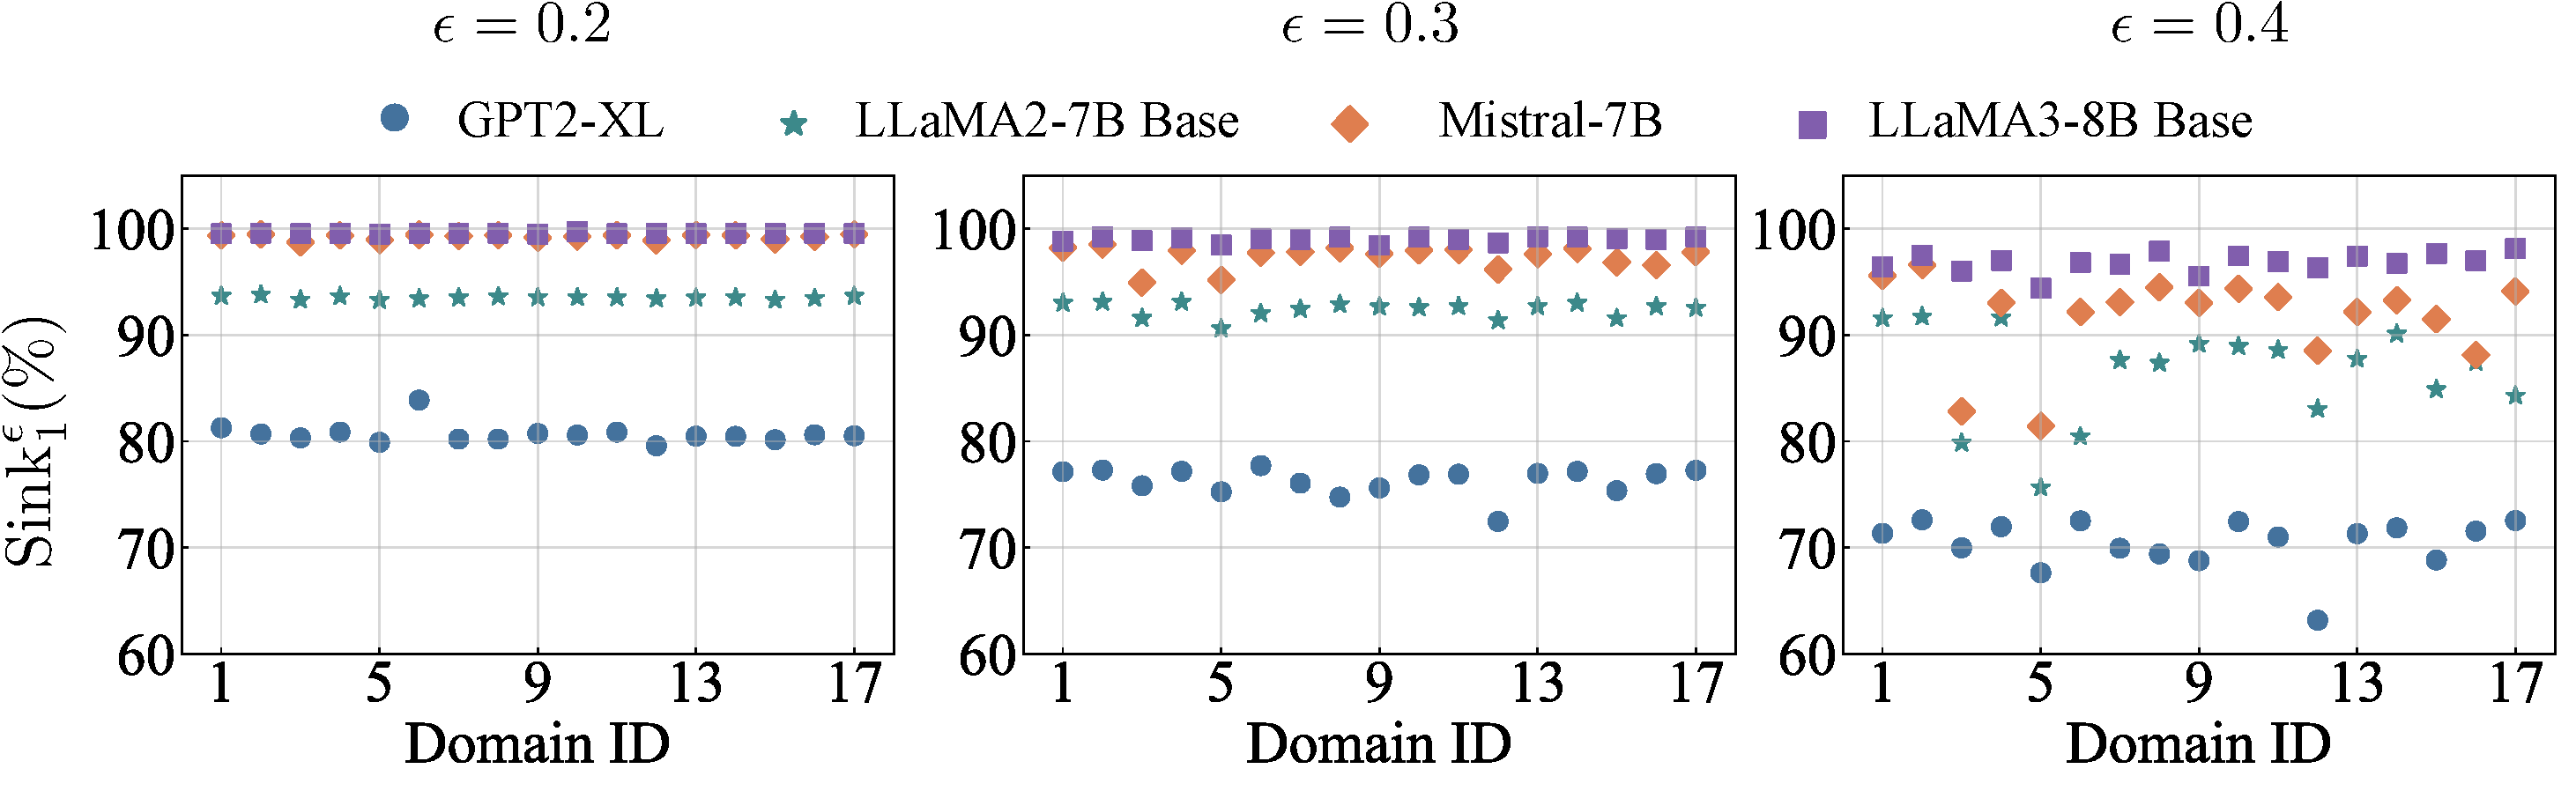
\includegraphics[width=\textwidth]{figures/attention_sink_domains.pdf}
\vspace{-0.2cm}
\caption{Input domains have negligible effects on attention sink metric $\textrm{Sink}_1^{\epsilon}$ for (\emph{left}) $\epsilon=\textrm{0.2}$ and (\emph{middle}) $\epsilon=\textrm{0.3}$. There are small fluctuations for (\emph{right}) $\epsilon=\textrm{0.4}$.}
\vspace{-0.2cm}
\label{all_domains}
\end{figure}


\subsection{Attention sink under different pre-trained LMs}\label{vis_norm}

\textbf{Relation to LM performance.} We leverage the platform~\citep{eval-harness} to evaluate the performance of open-sourced LMs, including LLaMA2/LLaMA3/OPT/Pythia/GPT2 families, on downstream LM task, e.g., HellaSwag~\citep{zellers2019hellaswag}. The results are visualized parallel with our attention sink metric in Figure~\ref{lm_performance}, including both accuracy (Acc) and accuracy under normalization (Acc\_Norm). We find that within the same LM family, with the increase of model scale, both attention sink amplitude and downstream LM performance are increasing. However, across different LM families, stronger attention sink does not always correlate with better performance. For instance, the OPT family has stronger attention sink than Pythia under the comparable model scale. However, the downstream LM performance is comparable. 

\begin{figure}[htbp]
\centering
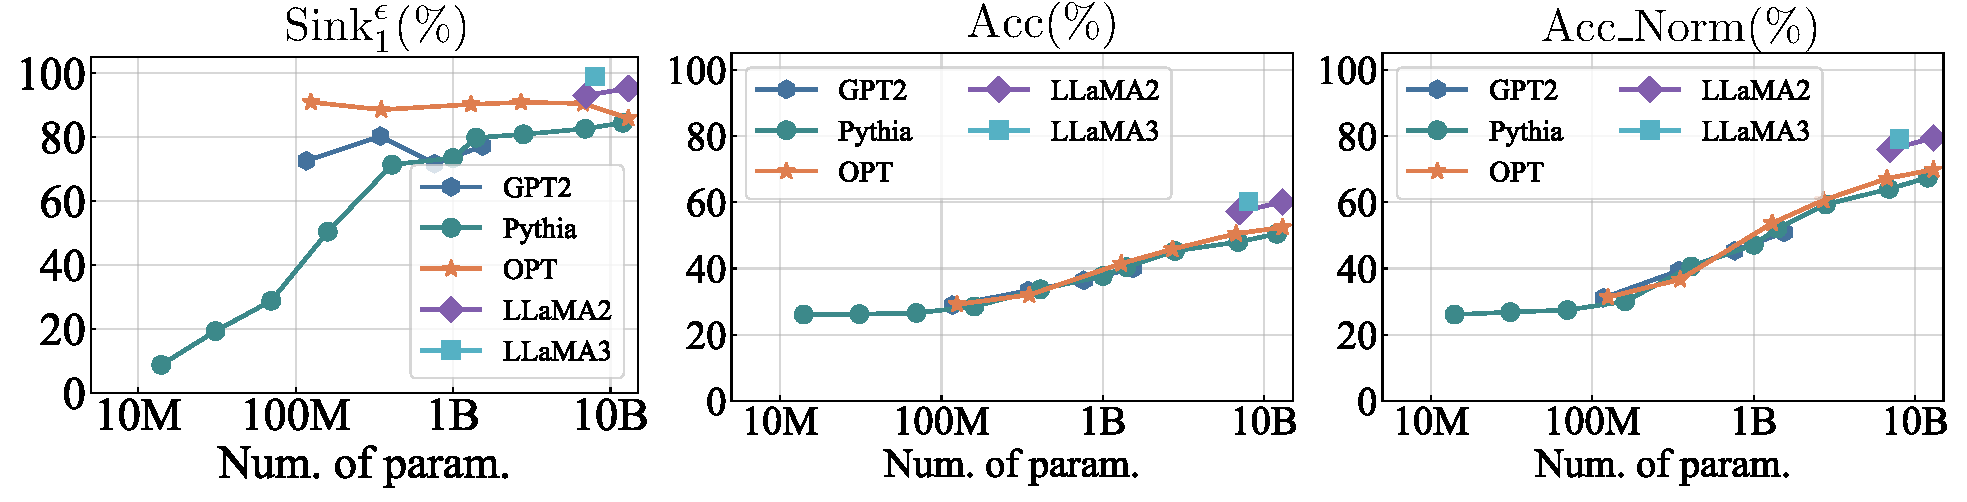
\includegraphics[width=\textwidth]{figures/hellaswag.pdf}
\vspace{-0.2cm}
\caption{Attention sink and downstream performance for various pre-trained LMs.}
\vspace{-0.2cm}
\label{lm_performance}
\end{figure}

\textbf{$\ell_2$-norm.} We first show that large $\ell_2$-norm of hidden states $\boldsymbol{h}_1^l$ and small $\ell_2$-norm of keys $\boldsymbol{k}_1^{l\textrm{,}\,h}$ and values $\boldsymbol{v}_1^{l\textrm{,}\,h}$ (especially for values) universally exist in open-sourced LMs, including LLaMA2-7B Base (Figure~\ref{appendix_l2_norm_llama2_7b}), GPT2-Large (Figure~\ref{appendix_l2_norm_gpt2_large}), Mistral-7B (Figure~\ref{appendix_l2_norm_mistral7b}), and Pythia-1B (Figure~\ref{appendix_l2_norm_pythia_1b}). It is noted that for the final transformer block $l=L$, we take the hidden states before LN. We note that different LMs may have different starting blocks where massive activations appear.\looseness=-1

% \clearpage
\begin{figure}[t]
\centering
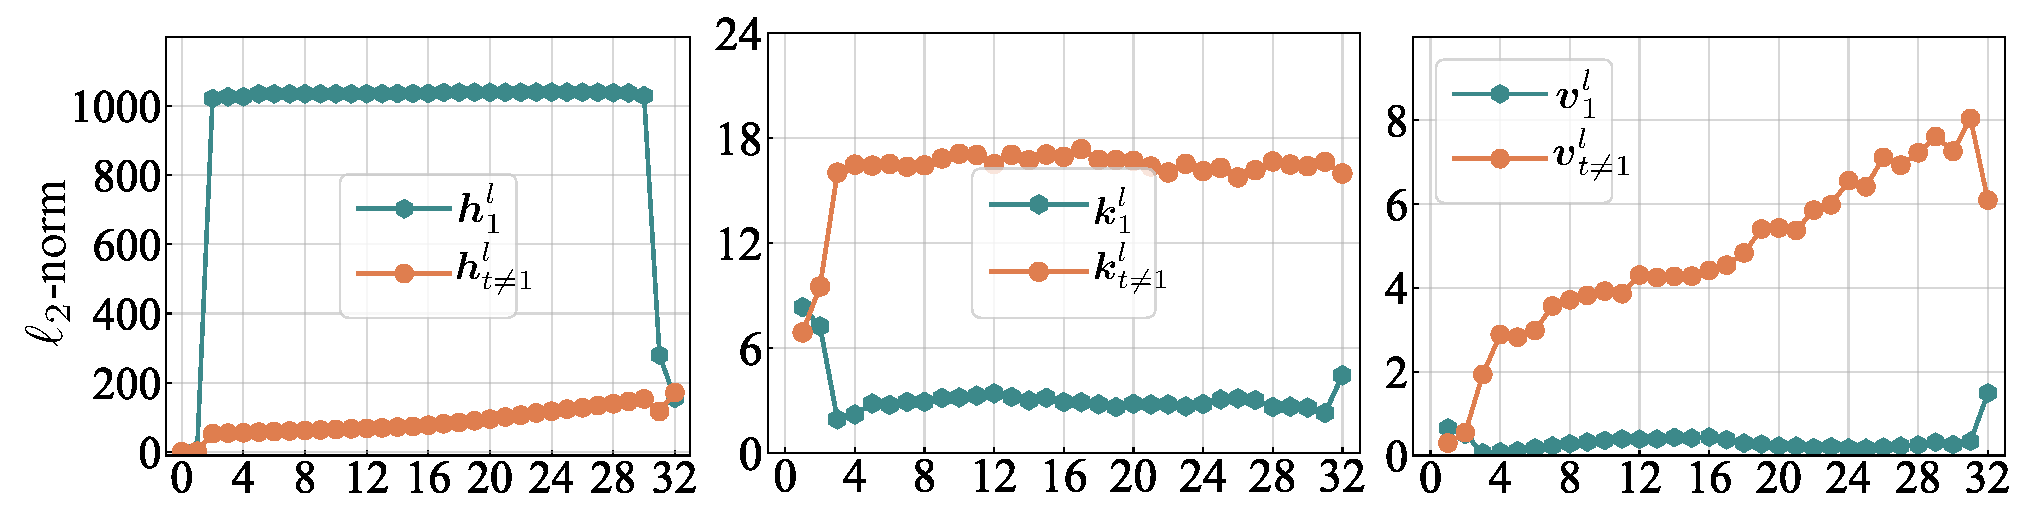
\includegraphics[width=\textwidth]{figures/appendix_l2_norm_llama2_7b_base.pdf}
% \vspace{-0.85cm}
\caption{$\ell_2$-norm of hidden states/keys/values of the first token/other tokens in LLaMA2-7B Base.\looseness=-1}
% \vspace{-0.2cm}
\label{appendix_l2_norm_llama2_7b}
\end{figure}

\begin{figure}[t]
\centering
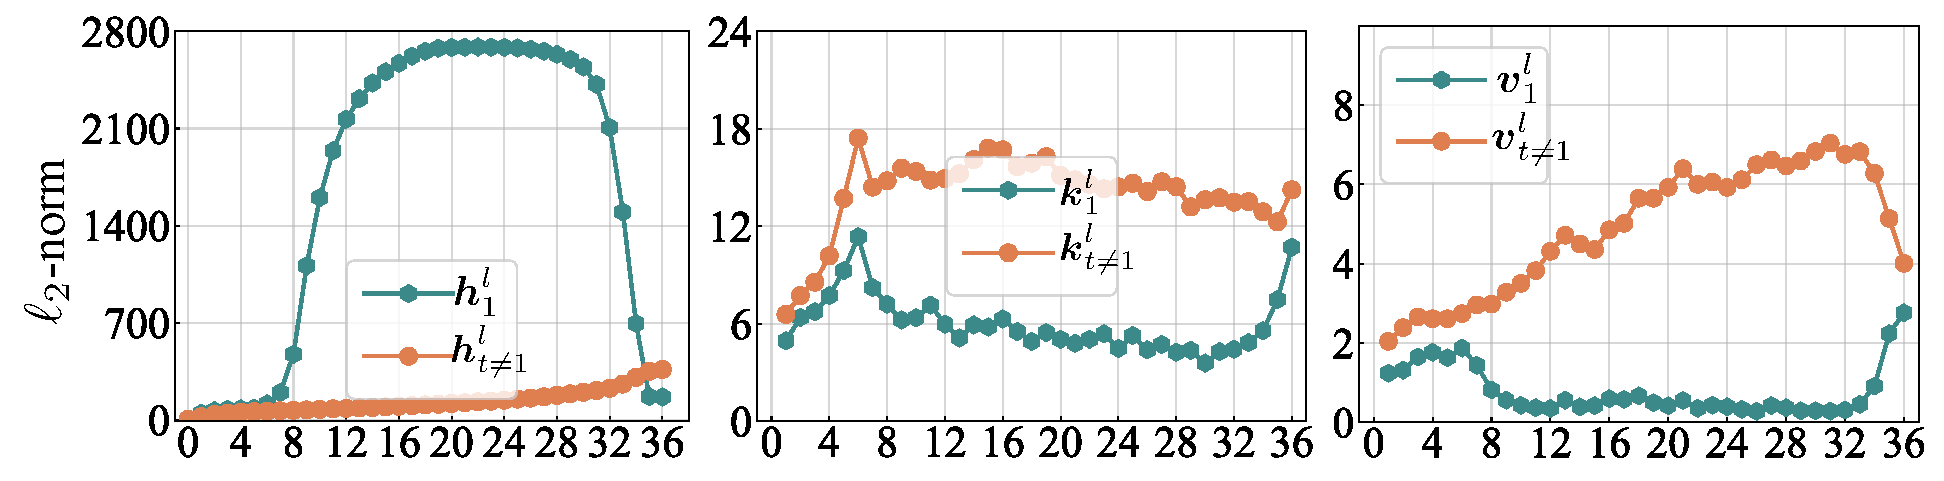
\includegraphics[width=\textwidth]{figures/appendix_l2_norm_gpt2_large.pdf}
\caption{$\ell_2$-norm of hidden states/keys/values of the first token/other tokens in GPT2-Large.\looseness=-1}
\label{appendix_l2_norm_gpt2_large}
\end{figure}

\begin{figure}[t]
\centering
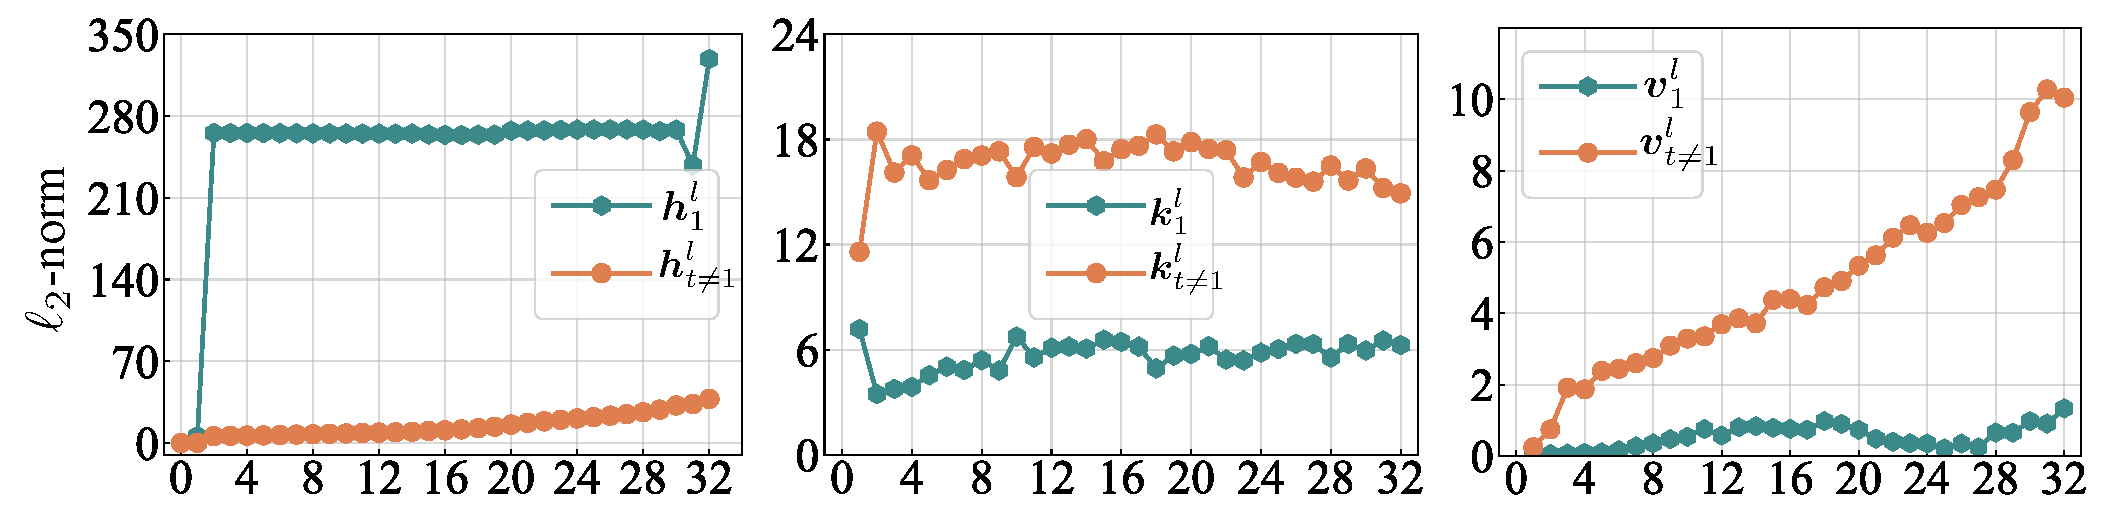
\includegraphics[width=\textwidth]{figures/appendix_l2_norm_mistral_7b_base.pdf}
\caption{$\ell_2$-norm of hidden states/keys/values of the first token/other tokens in Mistral-7B.\looseness=-1}
\label{appendix_l2_norm_mistral7b}
\end{figure}


\begin{figure}[t]
\centering
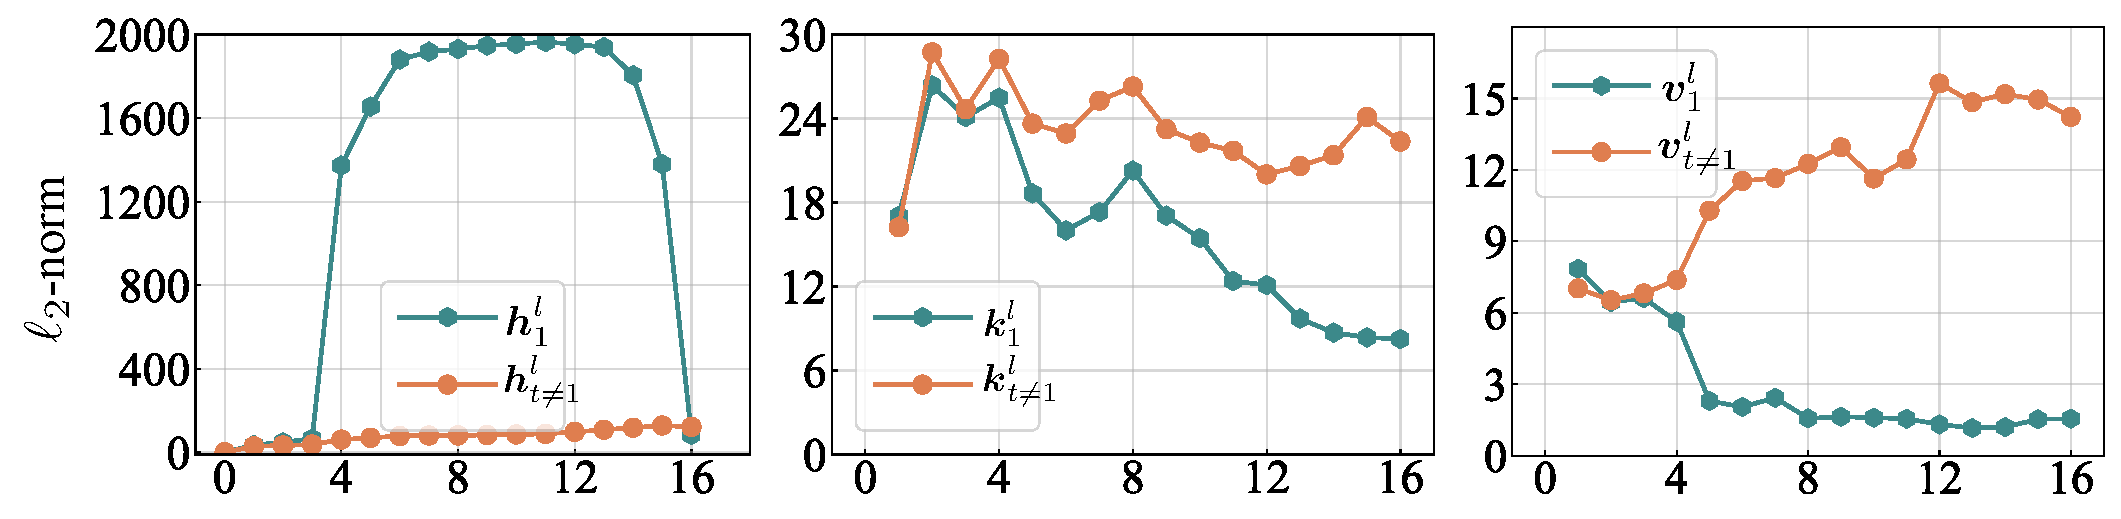
\includegraphics[width=\textwidth]{figures/appendix_l2_norm_pythia_1b.pdf}
\caption{$\ell_2$-norm of hidden states/keys/values of the first token/other tokens in Pythia-1B.\looseness=-1}
\label{appendix_l2_norm_pythia_1b}
\end{figure}

% \begin{figure}[t]
% \centering
% 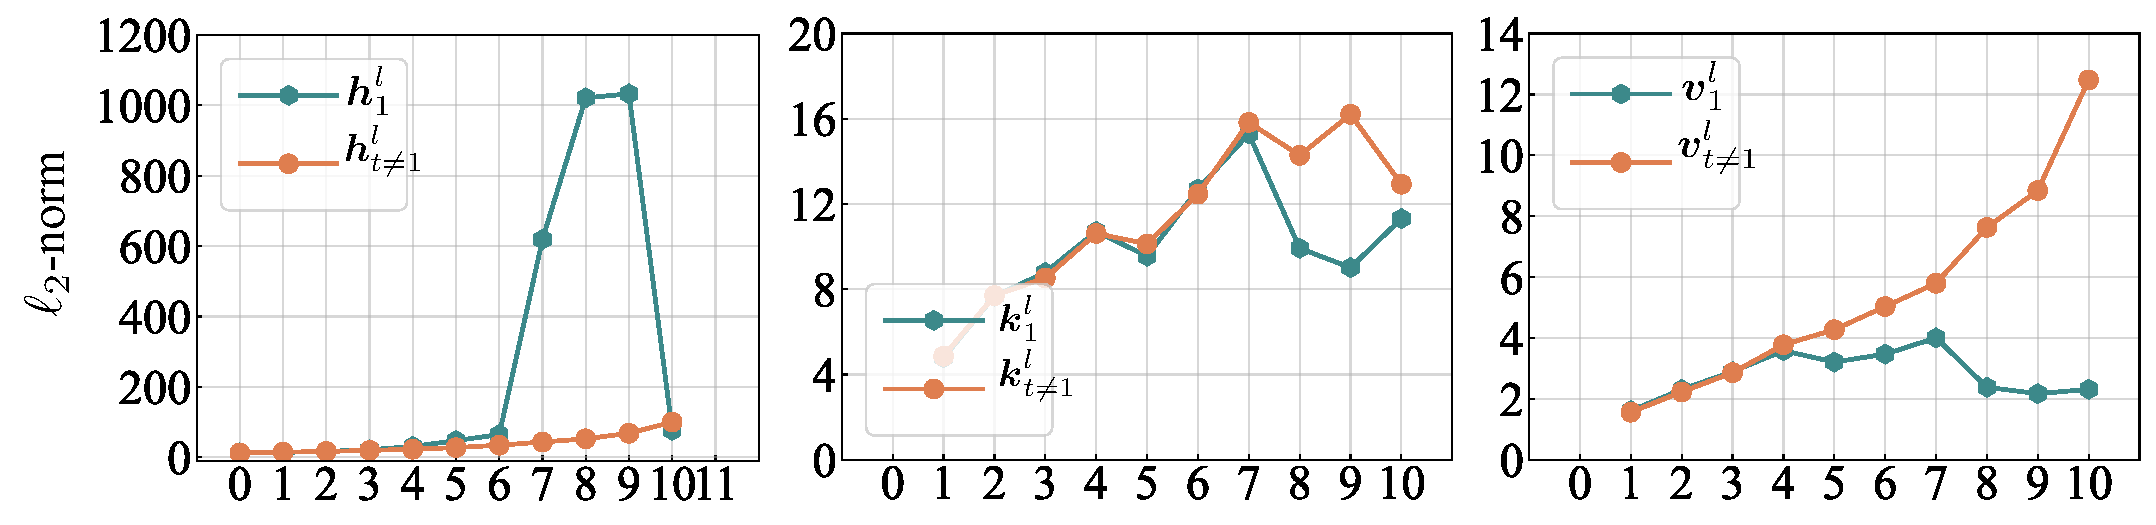
\includegraphics[width=\textwidth]{figures/appendix_l2_norm_llama_60m.pdf}
% \caption{$\ell_2$-norm of hidden states/keys/values of the first token/other tokens in our LLaMA model.\looseness=-1}
% \label{appendix_l2_norm_tinyllama}
% \end{figure}

\clearpage
\textbf{QK angles.} Then we further demonstrate that QK angles contribute to attention sink through more visualizations, including LLaMA3-8B Base (Figure~\ref{appendix_qk_angle_llama3_8b}), LLaMA2-7B Base (Figure~\ref{appendix_qk_angle_llama2_7b}), Mistral-7B (Figure~\ref{appendix_qk_angle_mistral_7b}), and GPT2-Large (Figure~\ref{appendix_qk_angle_gpt2_large}).


\begin{figure}[t]
\centering
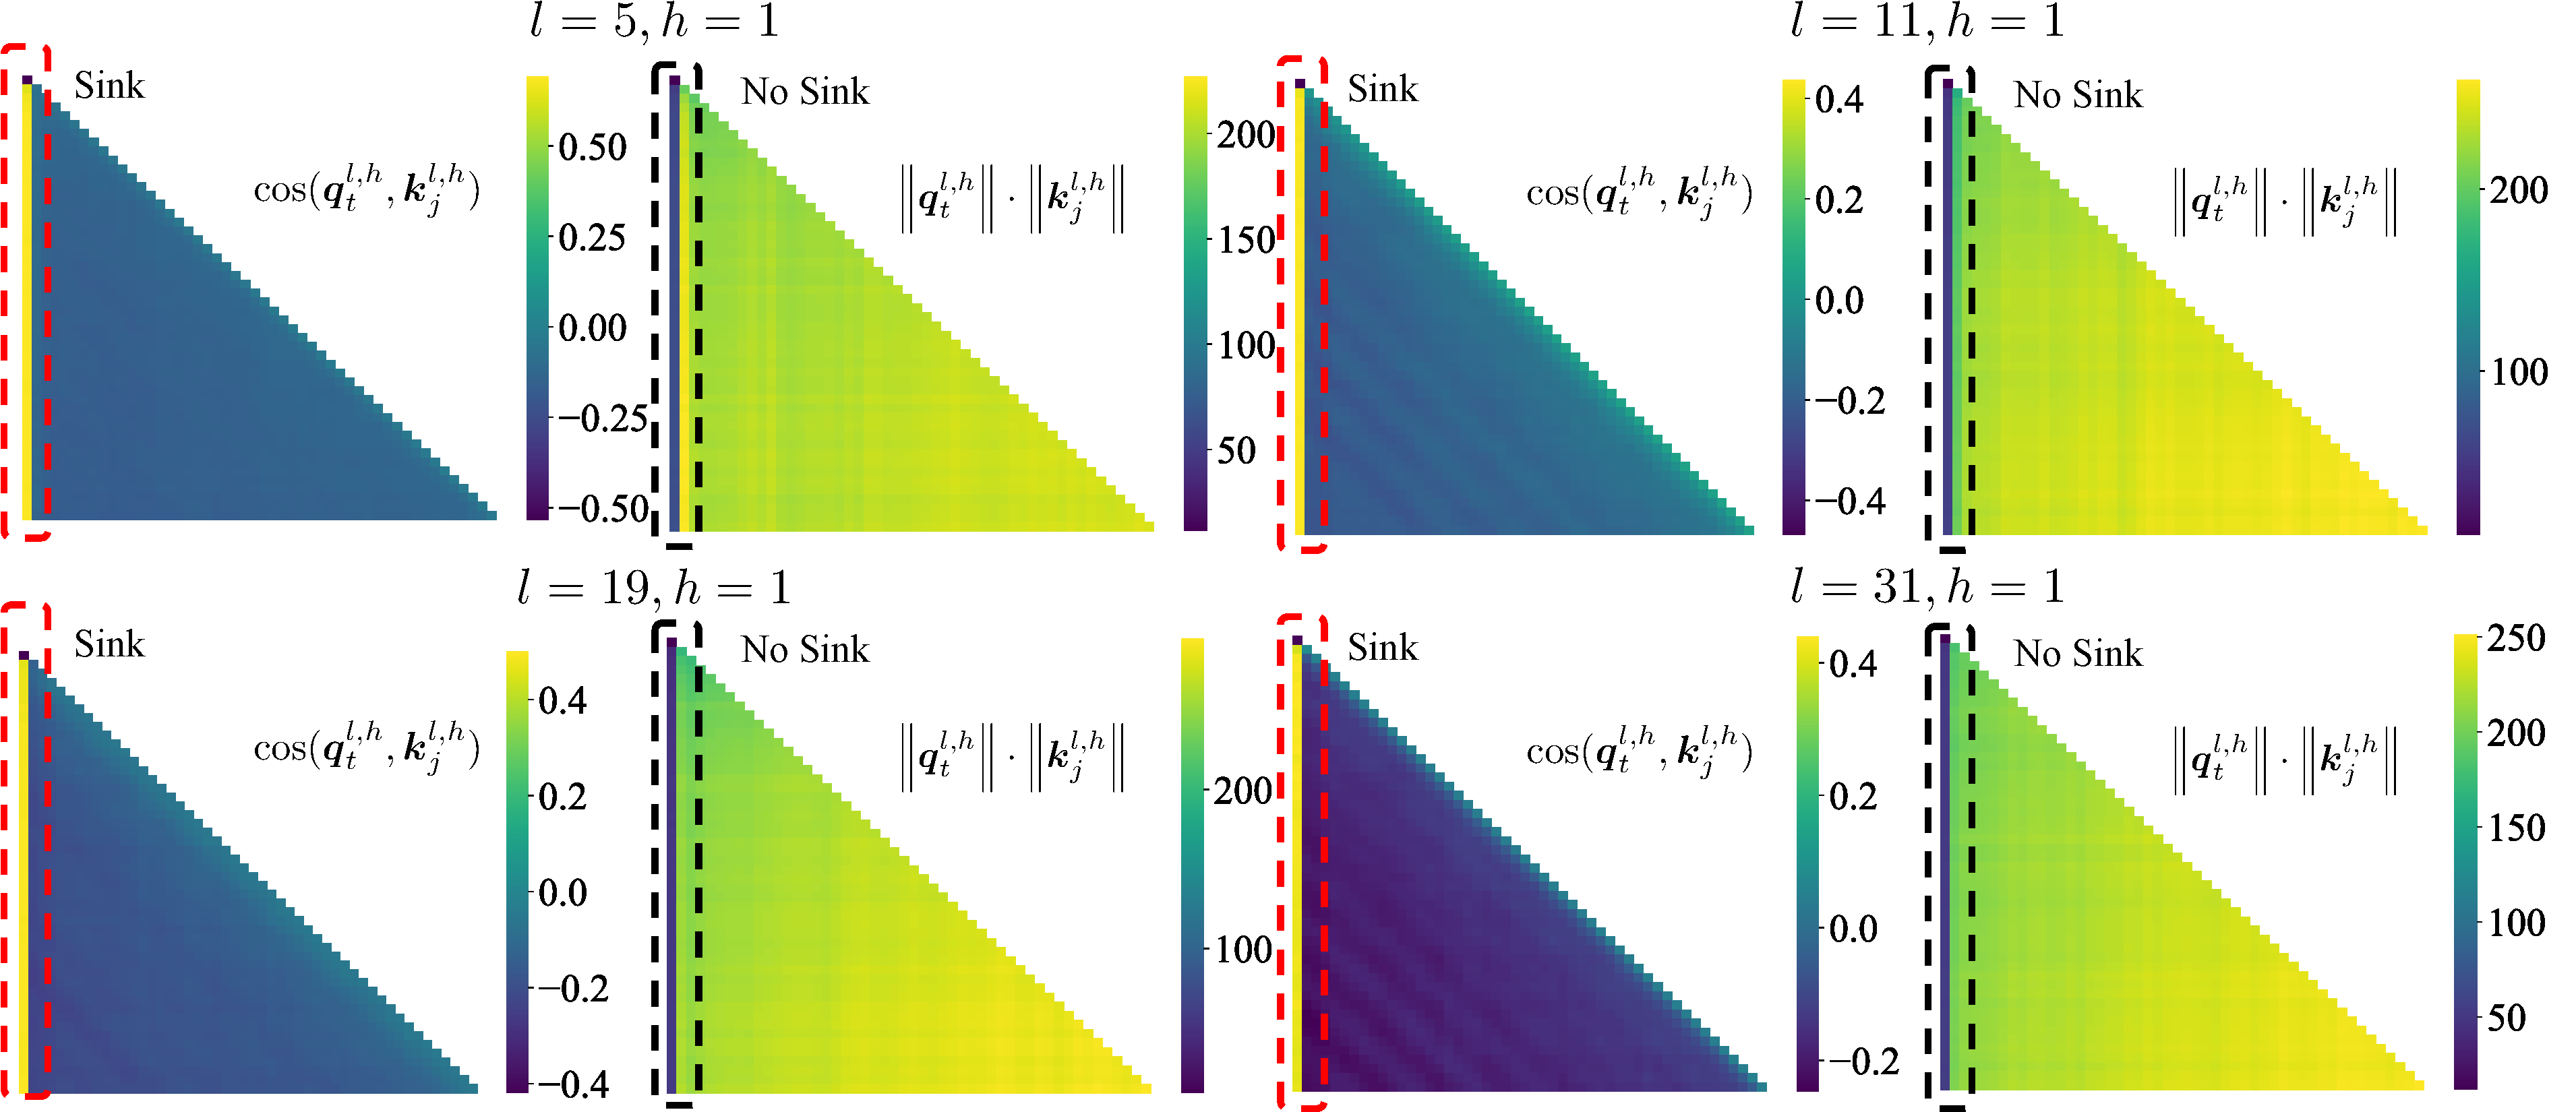
\includegraphics[width=\textwidth]{figures/appendix_qk_angle_llama3_8b_base.pdf}
% \vspace{-0.85cm}
\vspace{-0.2cm}
\caption{Cosine similarity and $\ell_2$-norm product between keys and queries in LLaMA3-8B Base.\looseness=-1}
\vspace{-0.2cm}
\label{appendix_qk_angle_llama3_8b}
\end{figure}

\begin{figure}[t]
\centering
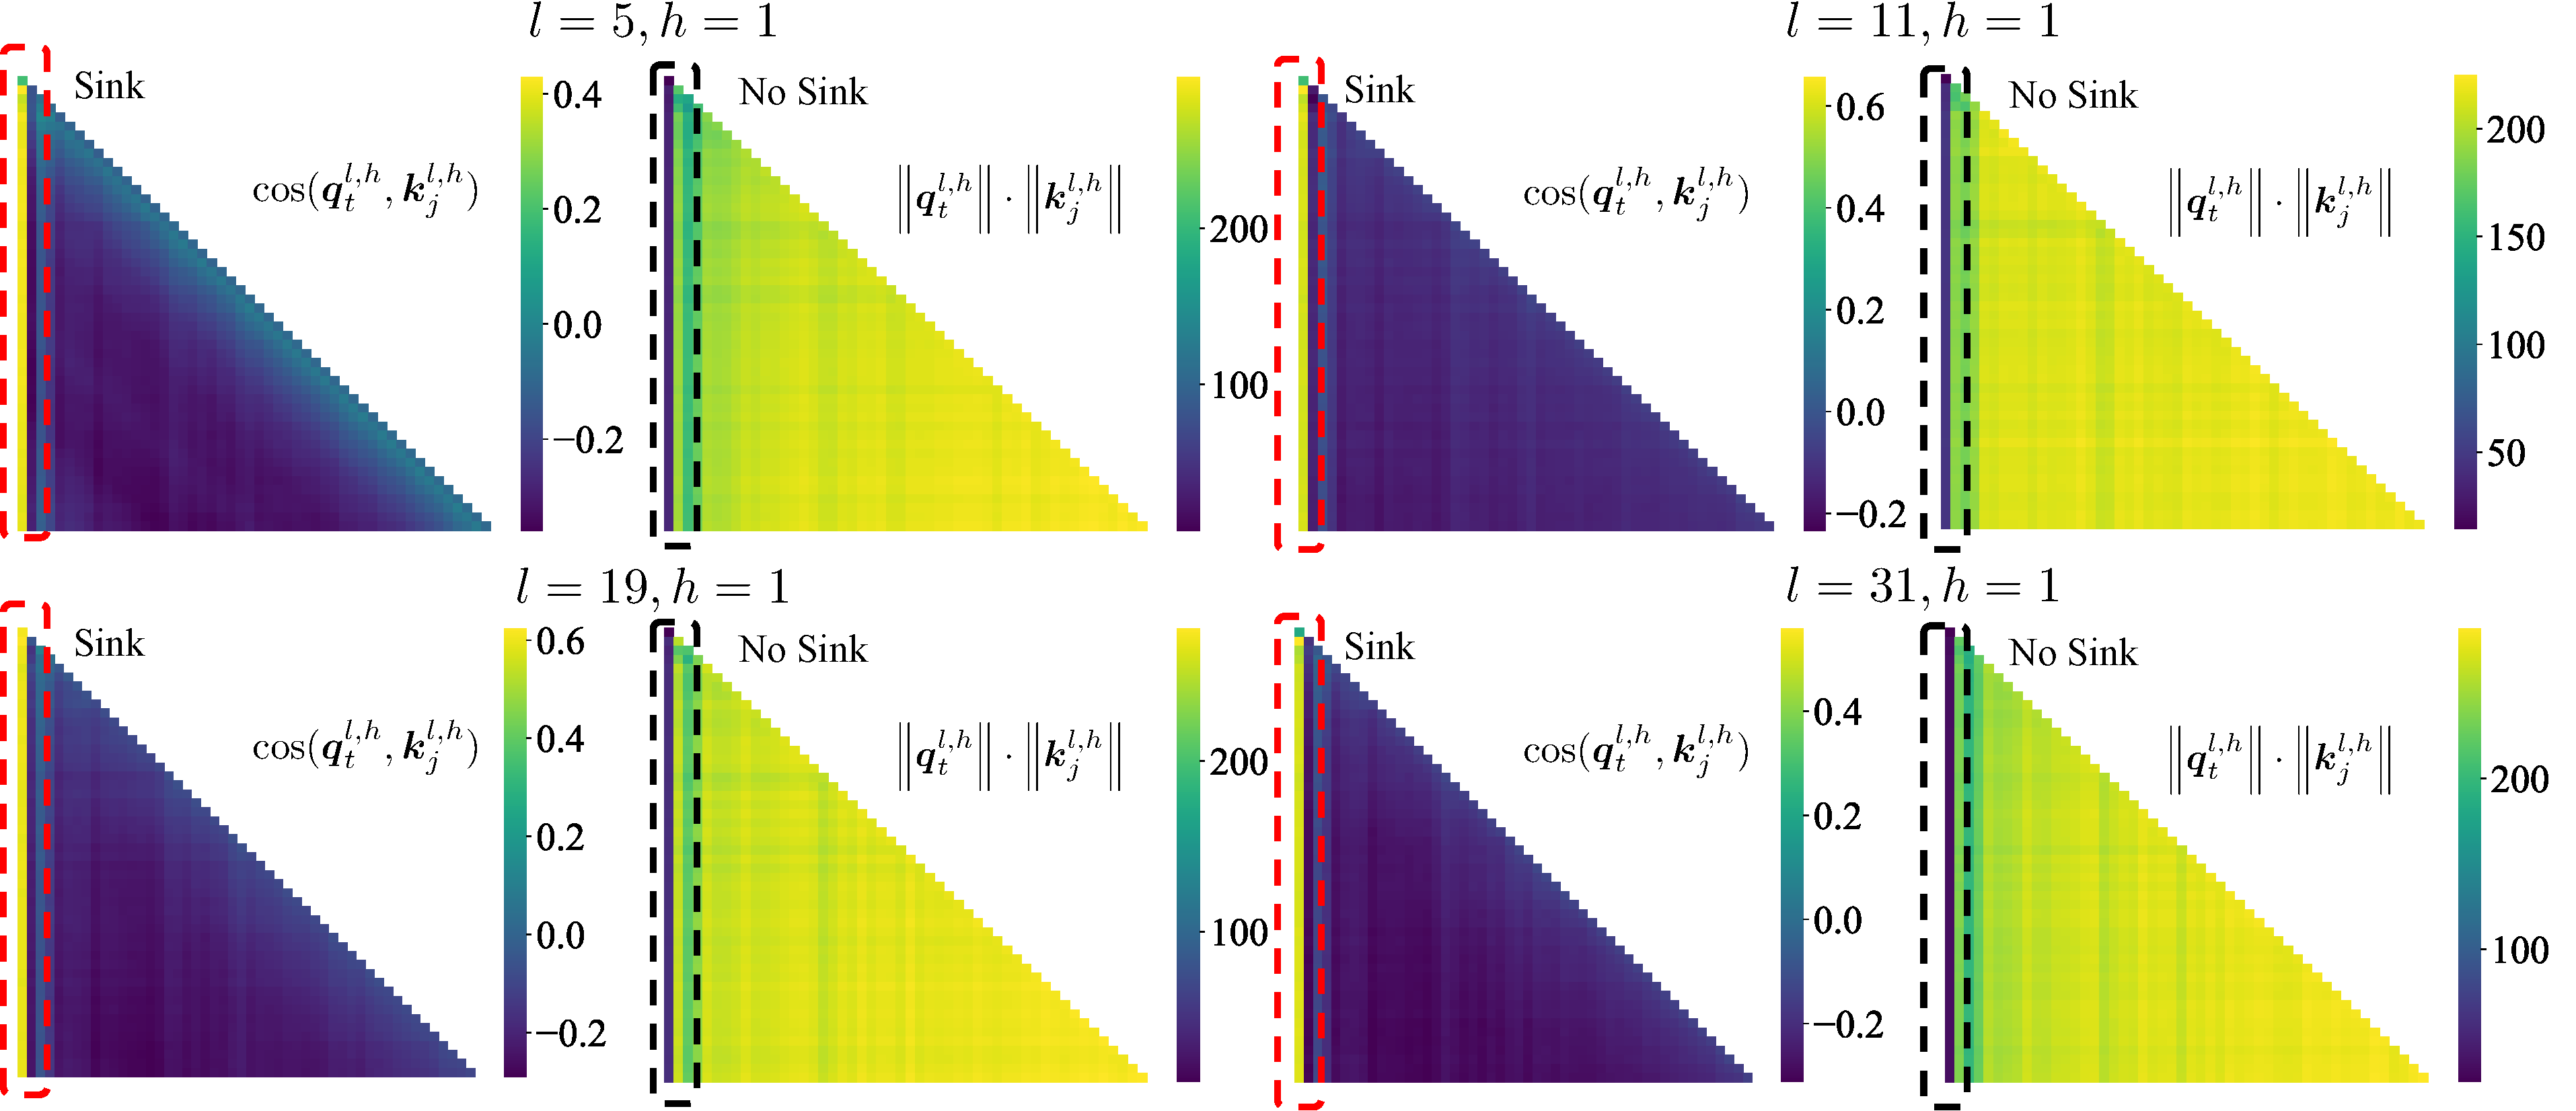
\includegraphics[width=\textwidth]{figures/appendix_qk_angle_llama2_7b_base.pdf}
% \vspace{-0.85cm}
\vspace{-0.2cm}
\caption{Cosine similarity and $\ell_2$-norm product between keys and queries in LLaMA2-7B Base.\looseness=-1}
\vspace{-0.2cm}
\label{appendix_qk_angle_llama2_7b}
\end{figure}

\begin{figure}[htbp]
\centering
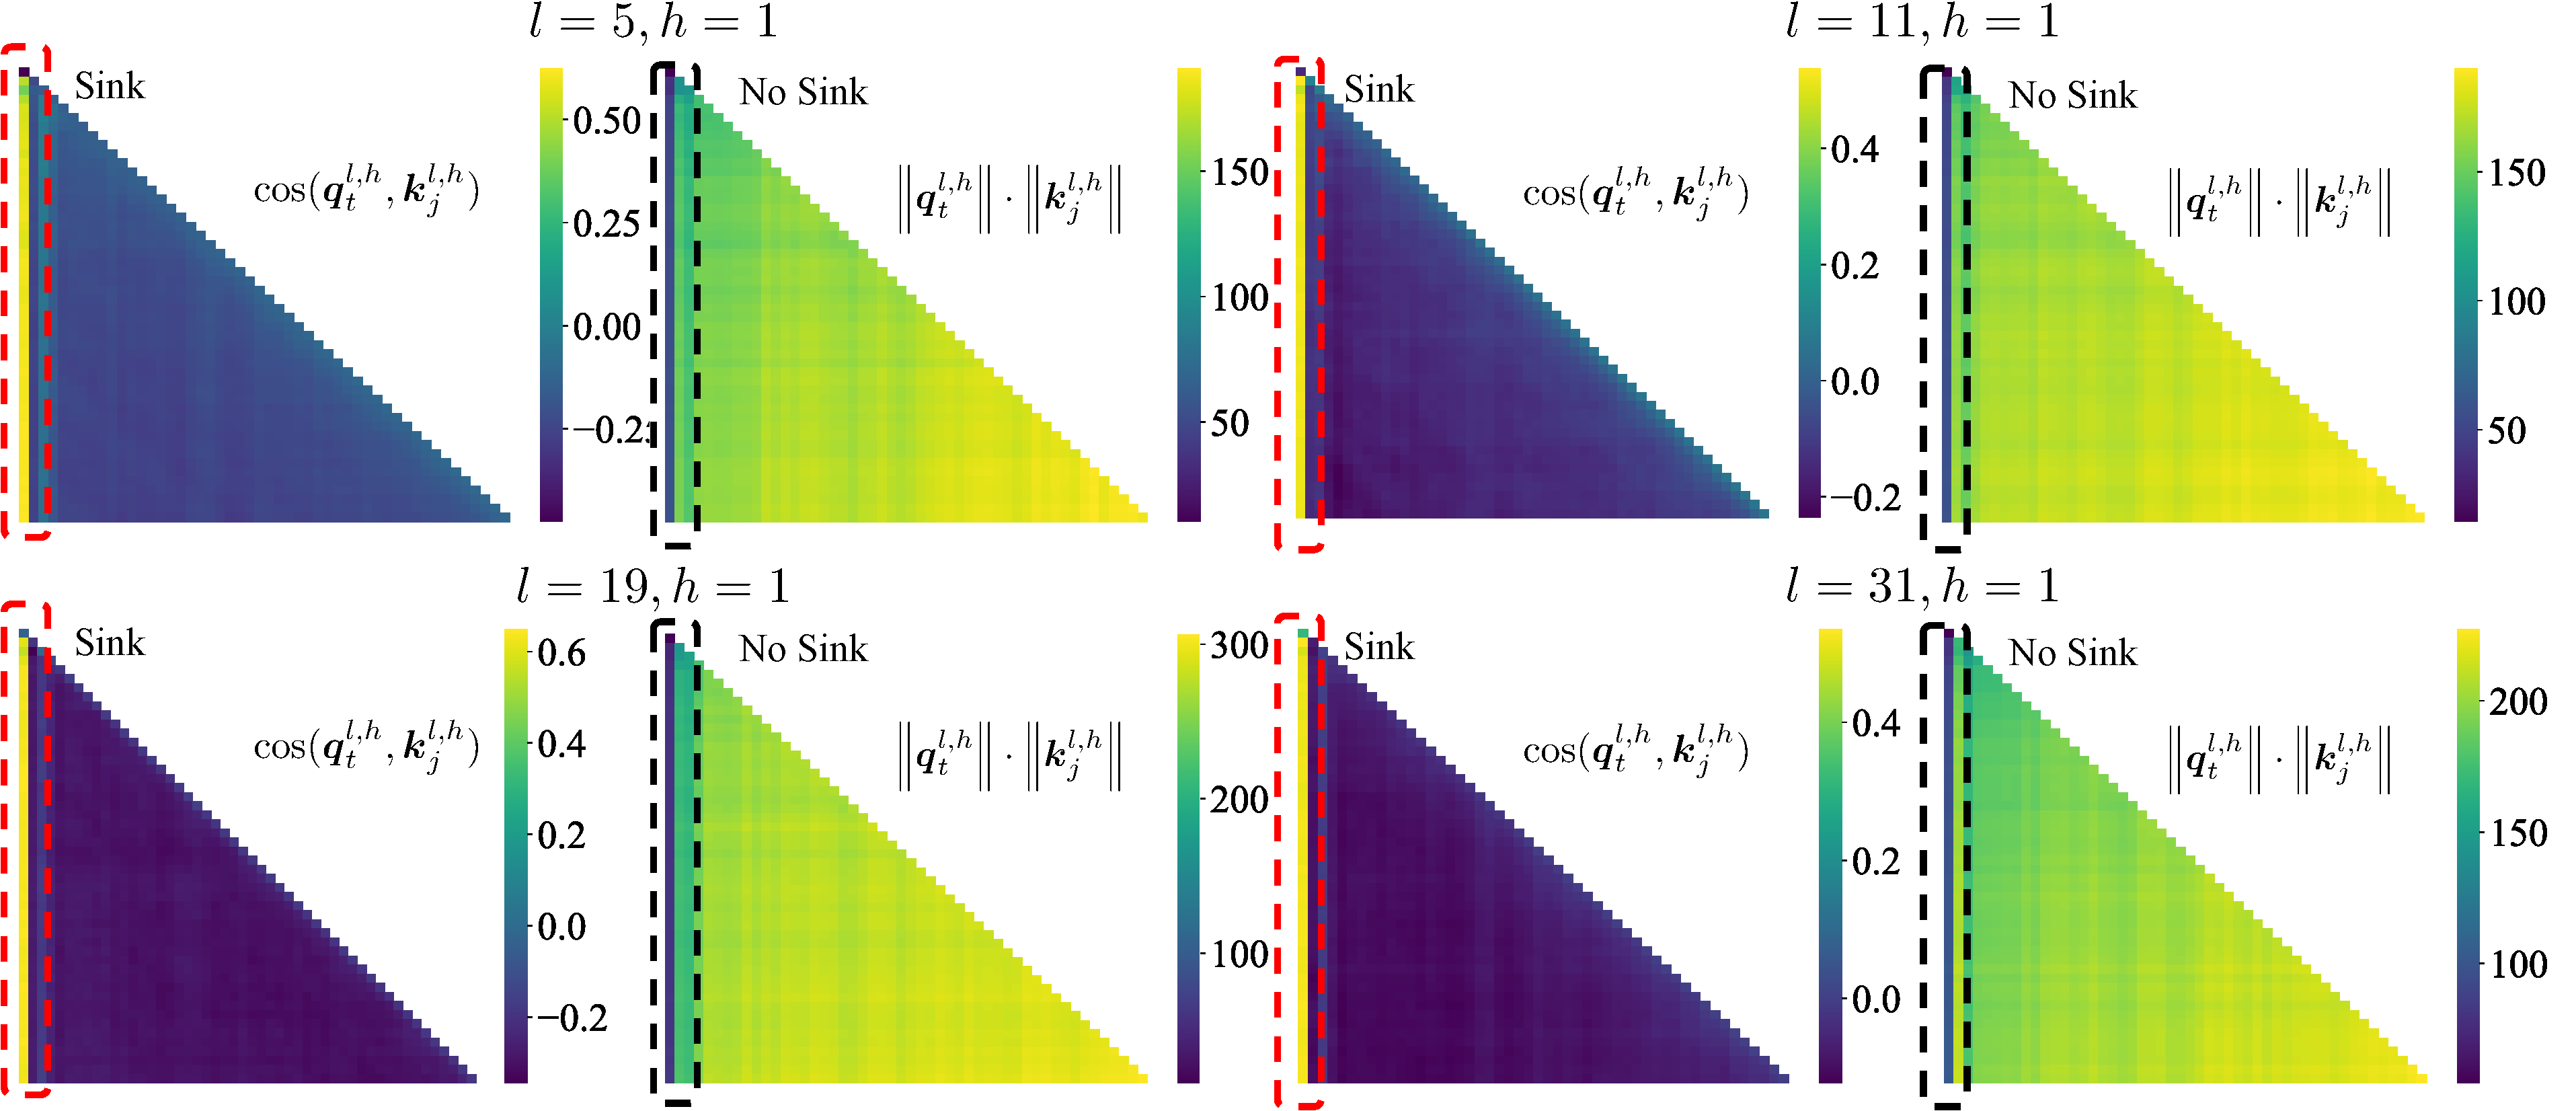
\includegraphics[width=\textwidth]{figures/appendix_qk_angle_mistral_7b_base.pdf}
% \vspace{-0.85cm}
\vspace{-0.2cm}
\caption{Cosine similarity and $\ell_2$-norm product between keys and queries in Mistral-7B.\looseness=-1}
\vspace{-0.2cm}
\label{appendix_qk_angle_mistral_7b}
\end{figure}

\begin{figure}[htbp]
\centering
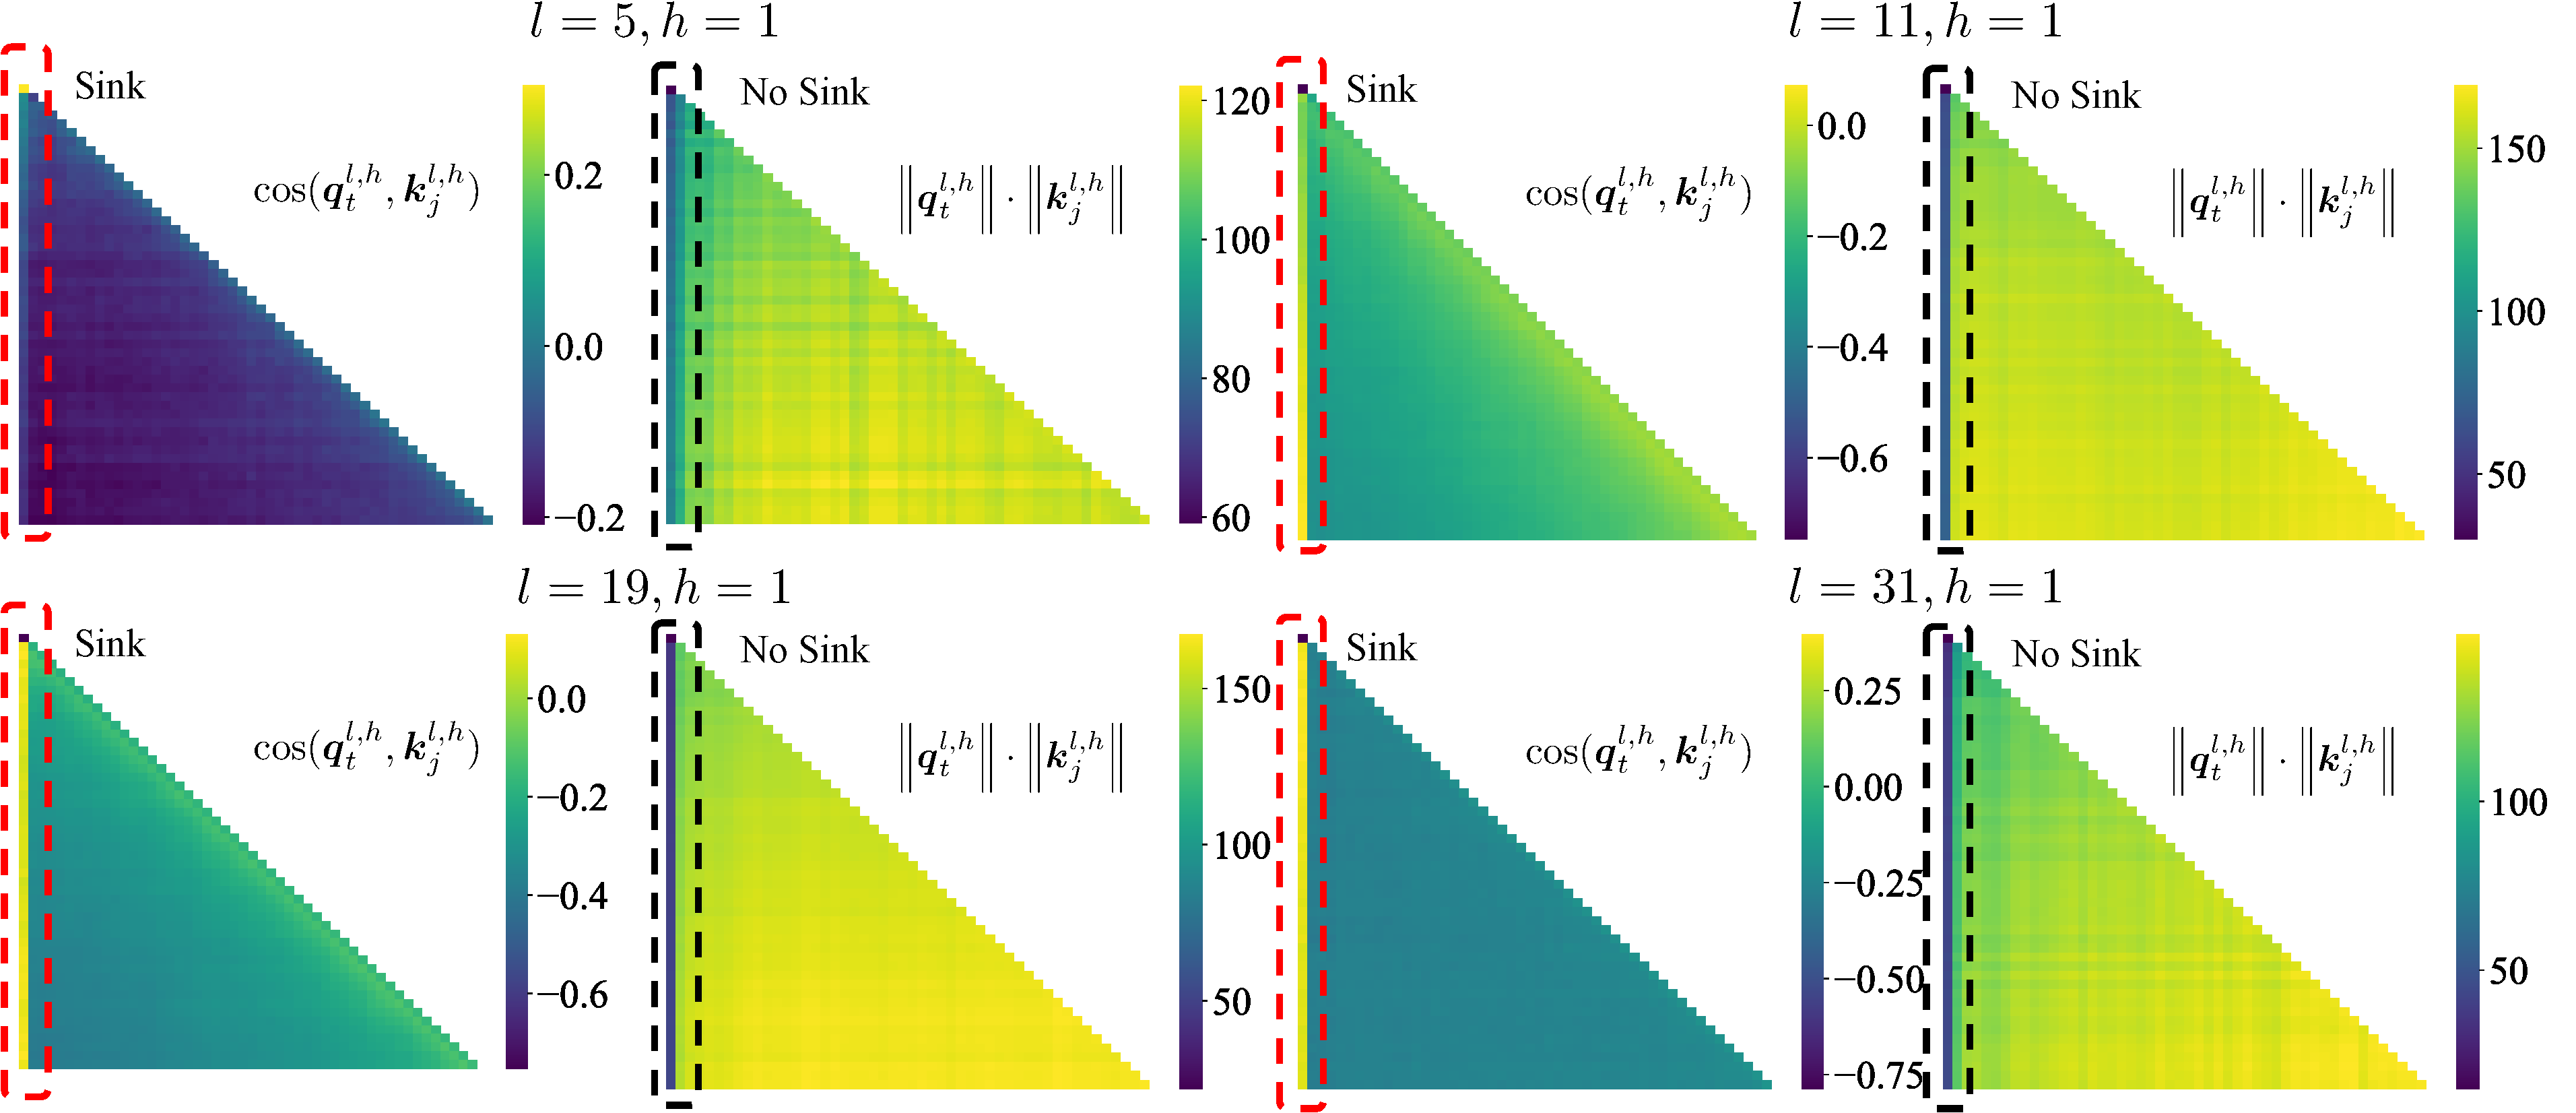
\includegraphics[width=\textwidth]{figures/appendix_qk_angle_gpt2_large.pdf}
% \vspace{-0.85cm}
\vspace{-0.2cm}
\caption{Cosine similarity and $\ell_2$-norm product between keys and queries in GPT2-Large.\looseness=-1}
\vspace{-0.2cm}
\label{appendix_qk_angle_gpt2_large}
\end{figure}

\textbf{Block-wise and head-wise property.} In the main paper, we mainly discuss the ratio of heads that have attention sink in the definition of attention sink metric $\textrm{Sink}_k^{\epsilon}$. Here we visualize the locations of these attention sink heads in open-sourced LMs, including LLaMA2 family (Figure~\ref{appendix_layer_head_llama2}), LLaMA3/LLaMA3.1 family (Figure~\ref{appendix_layer_head_llama3}), Mistral family (Figure~\ref{appendix_layer_head_mistral}), GPT2 family (Figure~\ref{appendix_layer_head_gpt2}), Pythia family (Figure~\ref{appendix_layer_head_pythia}), and OPT family (Figure~\ref{appendix_layer_head_opt}). We visualize the distributions of importance scores for the first token $\alpha_1^{l\textrm{,}\,h}$ across different transformer blocks $1 \leq l \leq L$ and different heads $1 \leq h \leq H$ before computing the attention sink metric. We find that (1) different pre-trained LMs have various attention sink distributions but they tend to have less obvious attention sink in earlier transformer blocks; (2) instruction tuning does not significantly modify such attention sink distributions when comparing base versions and chat/instruct versions.

\begin{figure}[htbp]
\centering
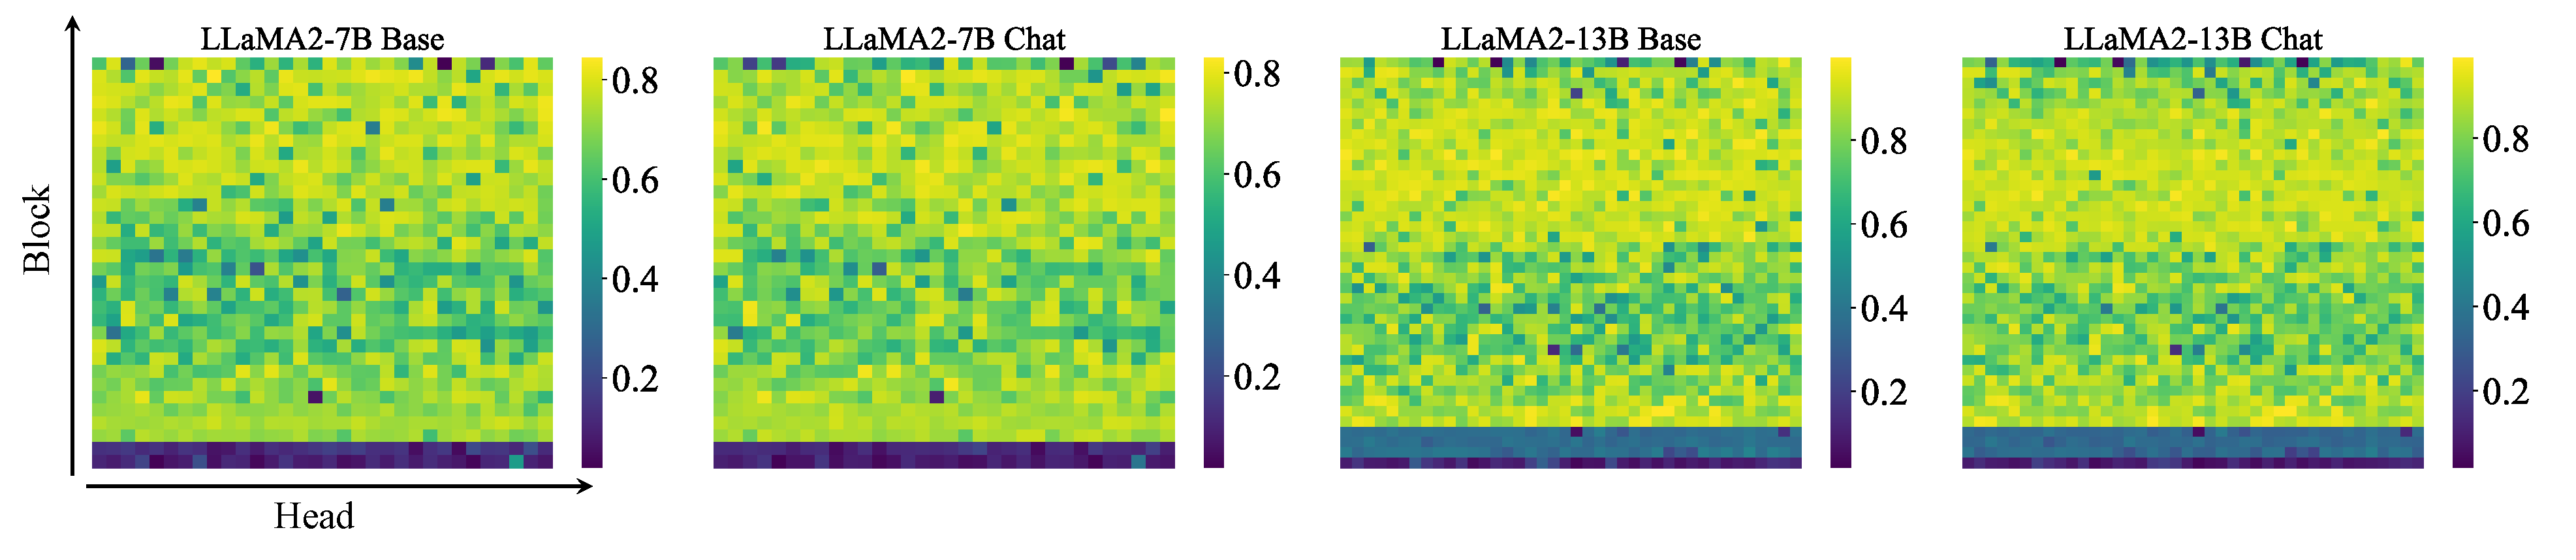
\includegraphics[width=\textwidth]{figures/appendix_layer_head_llama2.pdf}
% \vspace{-0.85cm}
% \vspace{-0.2cm}
\caption{Distribution of importance scores for the first token across different blocks and heads in the LLaMA2 family.\looseness=-1}
% \vspace{-0.2cm}
\label{appendix_layer_head_llama2}
\end{figure}

\begin{figure}[htbp]
\centering
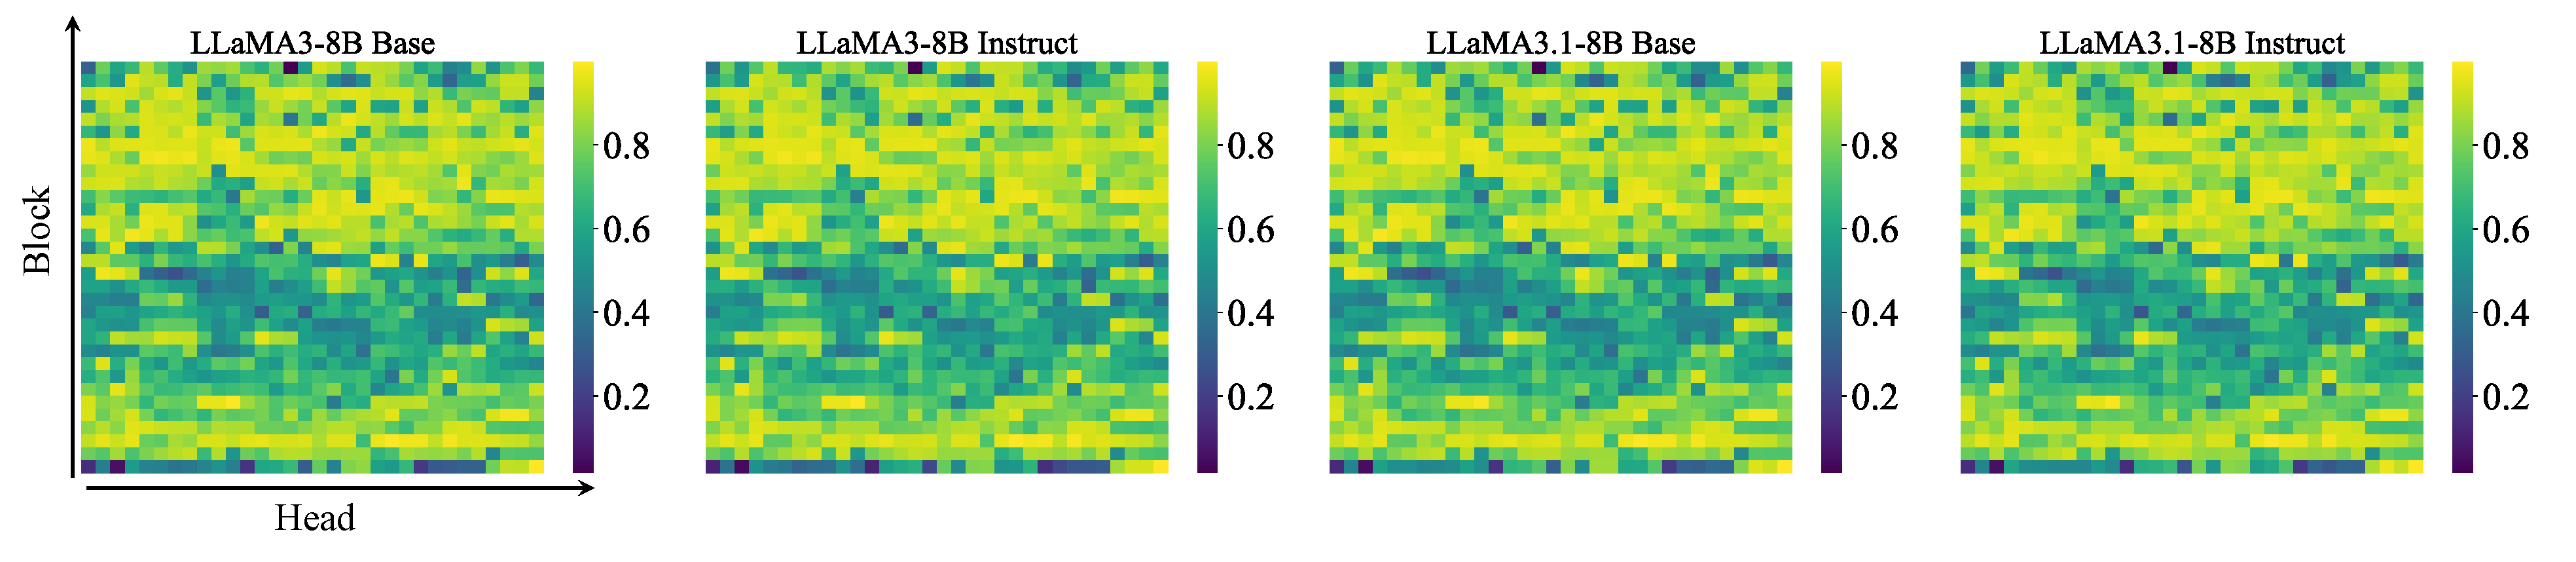
\includegraphics[width=\textwidth]{figures/appendix_layer_head_llama3.pdf}
% \vspace{-0.85cm}
% \vspace{-0.2cm}
\caption{Distribution of importance scores for the first token across blocks and heads in the LLaMA3/LLaMA3.1 family.\looseness=-1}
% \vspace{-0.2cm}
\label{appendix_layer_head_llama3}
\end{figure}


\begin{figure}[htbp]
\centering
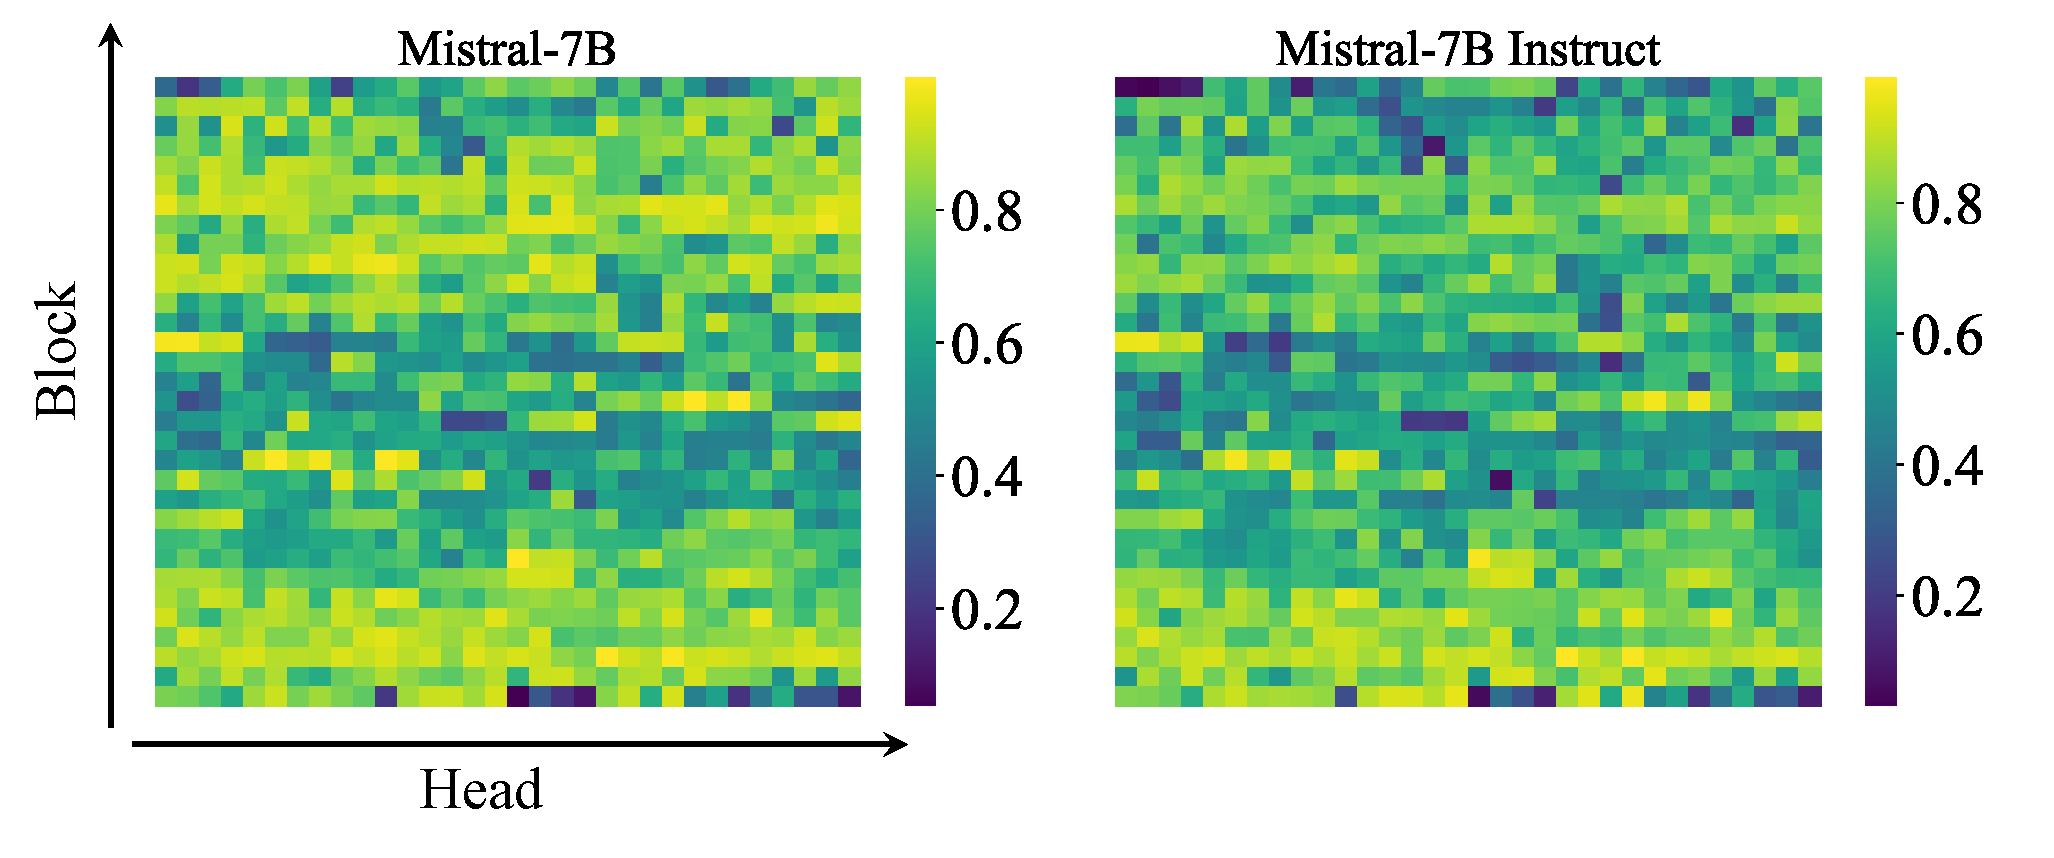
\includegraphics[width=0.5\textwidth]{figures/appendix_layer_head_mistral.pdf}
% \vspace{-0.85cm}
% \vspace{-0.3cm}
\caption{Distribution of importance scores for the first token across blocks and heads in the Mistral family.\looseness=-1}
% \vspace{-0.3cm}
\label{appendix_layer_head_mistral}
\end{figure}

\begin{figure}[htbp]
\centering
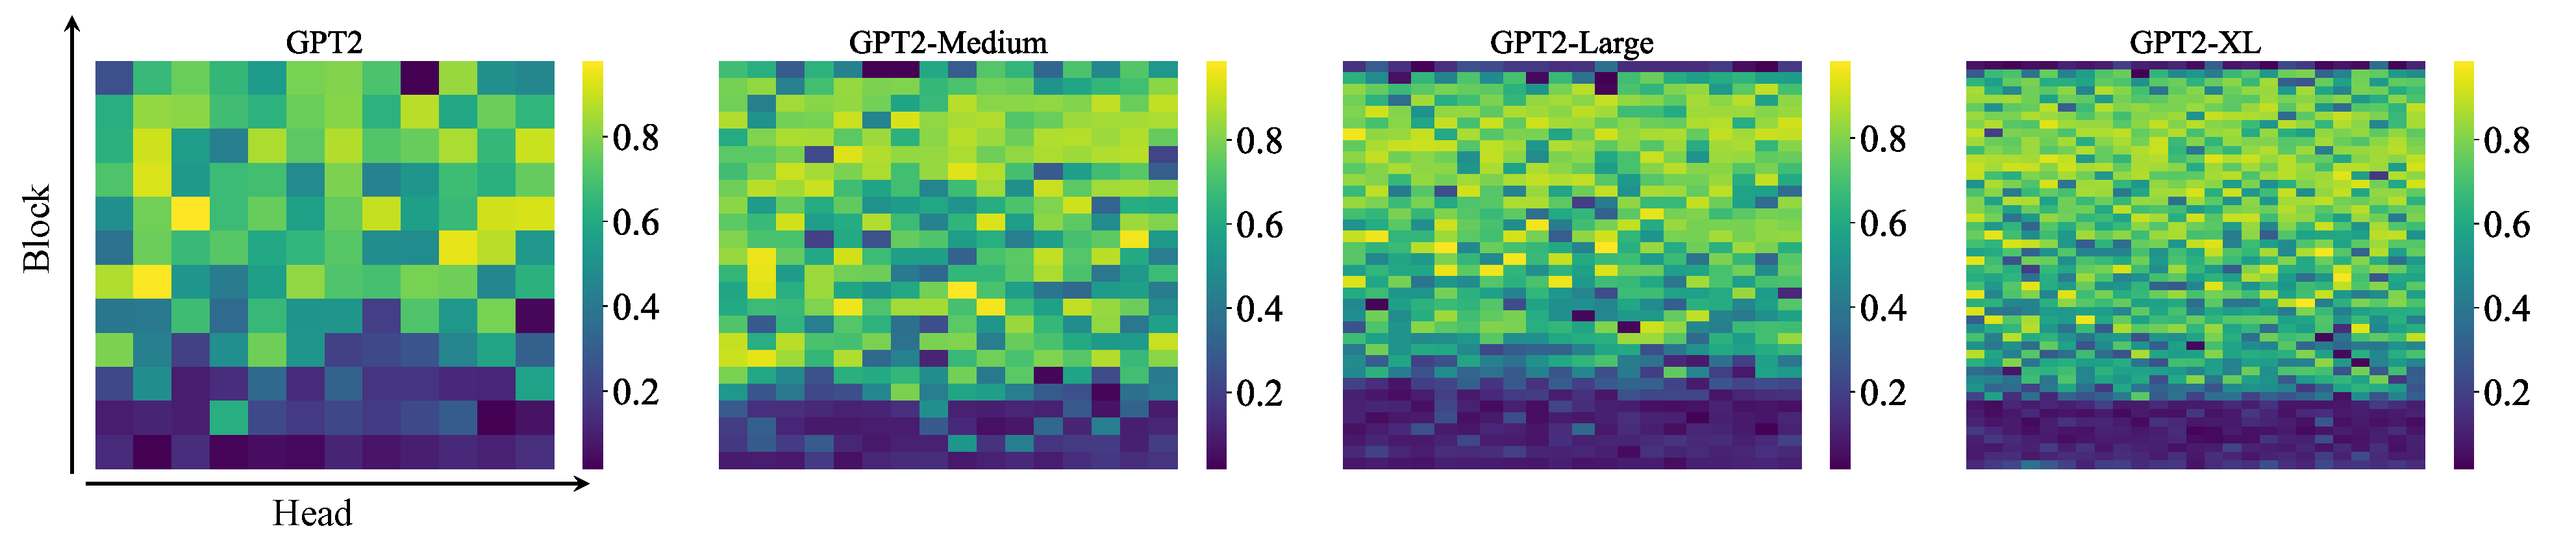
\includegraphics[width=\textwidth]{figures/appendix_layer_head_gpt2.pdf}
% \vspace{-0.85cm}
% \vspace{-0.3cm}
\caption{Distribution of importance scores for the first token across blocks and heads in the GPT2 family.\looseness=-1}
% \vspace{-0.3cm}
\label{appendix_layer_head_gpt2}
\end{figure}

\begin{figure}[htbp]
\centering
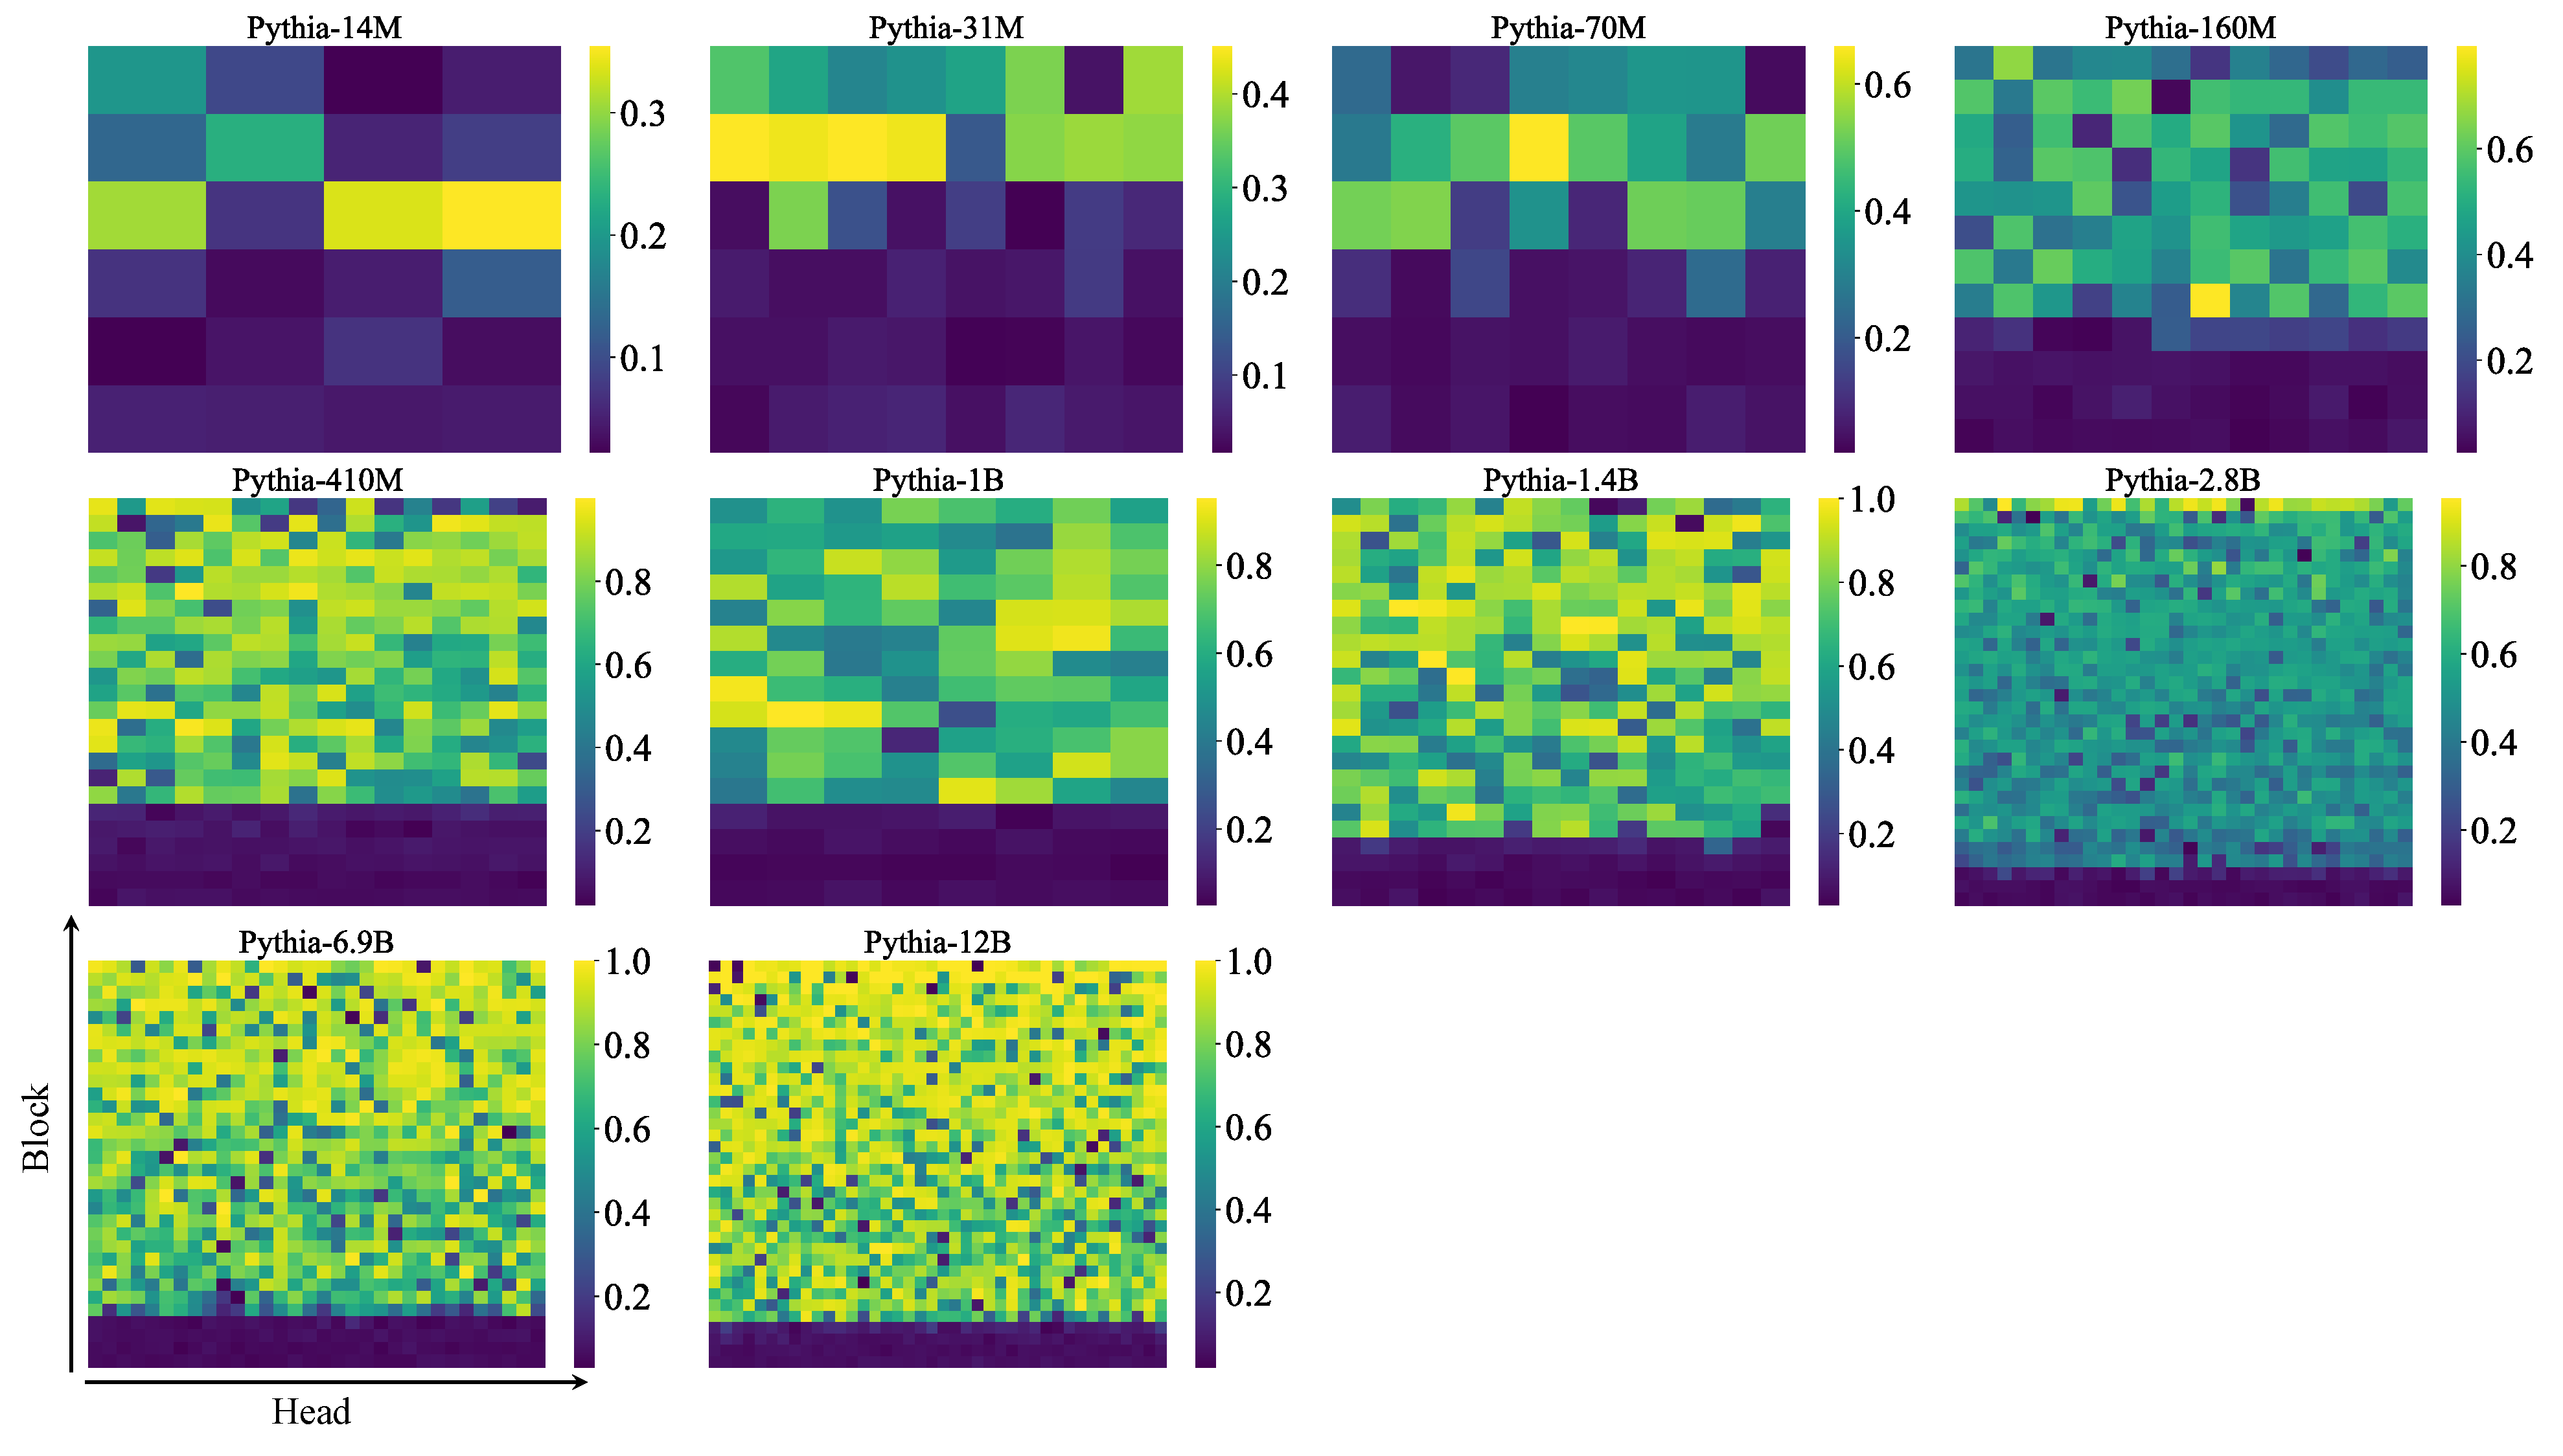
\includegraphics[width=\textwidth]{figures/appendix_layer_head_pythia.pdf}
% \vspace{-0.85cm}
% \vspace{-0.3cm}
\caption{Distribution of importance scores for the first token across blocks and heads in the Pythia family.\looseness=-1}
% \vspace{-0.3cm}
\label{appendix_layer_head_pythia}
\end{figure}


\clearpage

\textbf{Jamba.} Besides the auto-regressive Transformers, we also consider Jamba~\citep{lieber2024jamba,team2024jamba}, a new foundation language model. Both Jamba-v0.1~\citep{lieber2024jamba} and Jamba-1.5 Mini~\citep{team2024jamba} have 4 Jamba blocks, each of which includes 3 Mamba layers~\citep{gu2023mamba}, 4 Mamba MoE layers~\citep{shazeer2017outrageously, fedus2022switch}, and 1 Transformer layer. This adds to 32 layers (including 4 Transformer attention layers), 52B available parameters, and 12B active parameters in total. Firstly, we evaluate the attention sink metric and find that $\textrm{Sink}_1^{\epsilon}=\textrm{88.48}\%$ for Jamba-v0.1 and $\textrm{Sink}_1^{\epsilon}=\textrm{87.88}\%$ for Jamba-1.5 Mini, which indicates a strong attention sink on the first token. Then we visualize attention scores in several heads, as shown in Figure~\ref{appendix_sink_jamba_v0.1} and Figure~\ref{appendix_sink_jamba_1.5_mini}.  We also visualize the distribution of importance scores for the first token across blocks and heads in Jamba models in Figure~\ref{appendix_layer_head_jamba}. We observe that most heads have obvious attention sink, except for several heads in the 3rd Transformer layer.

\begin{figure}[t]
\centering
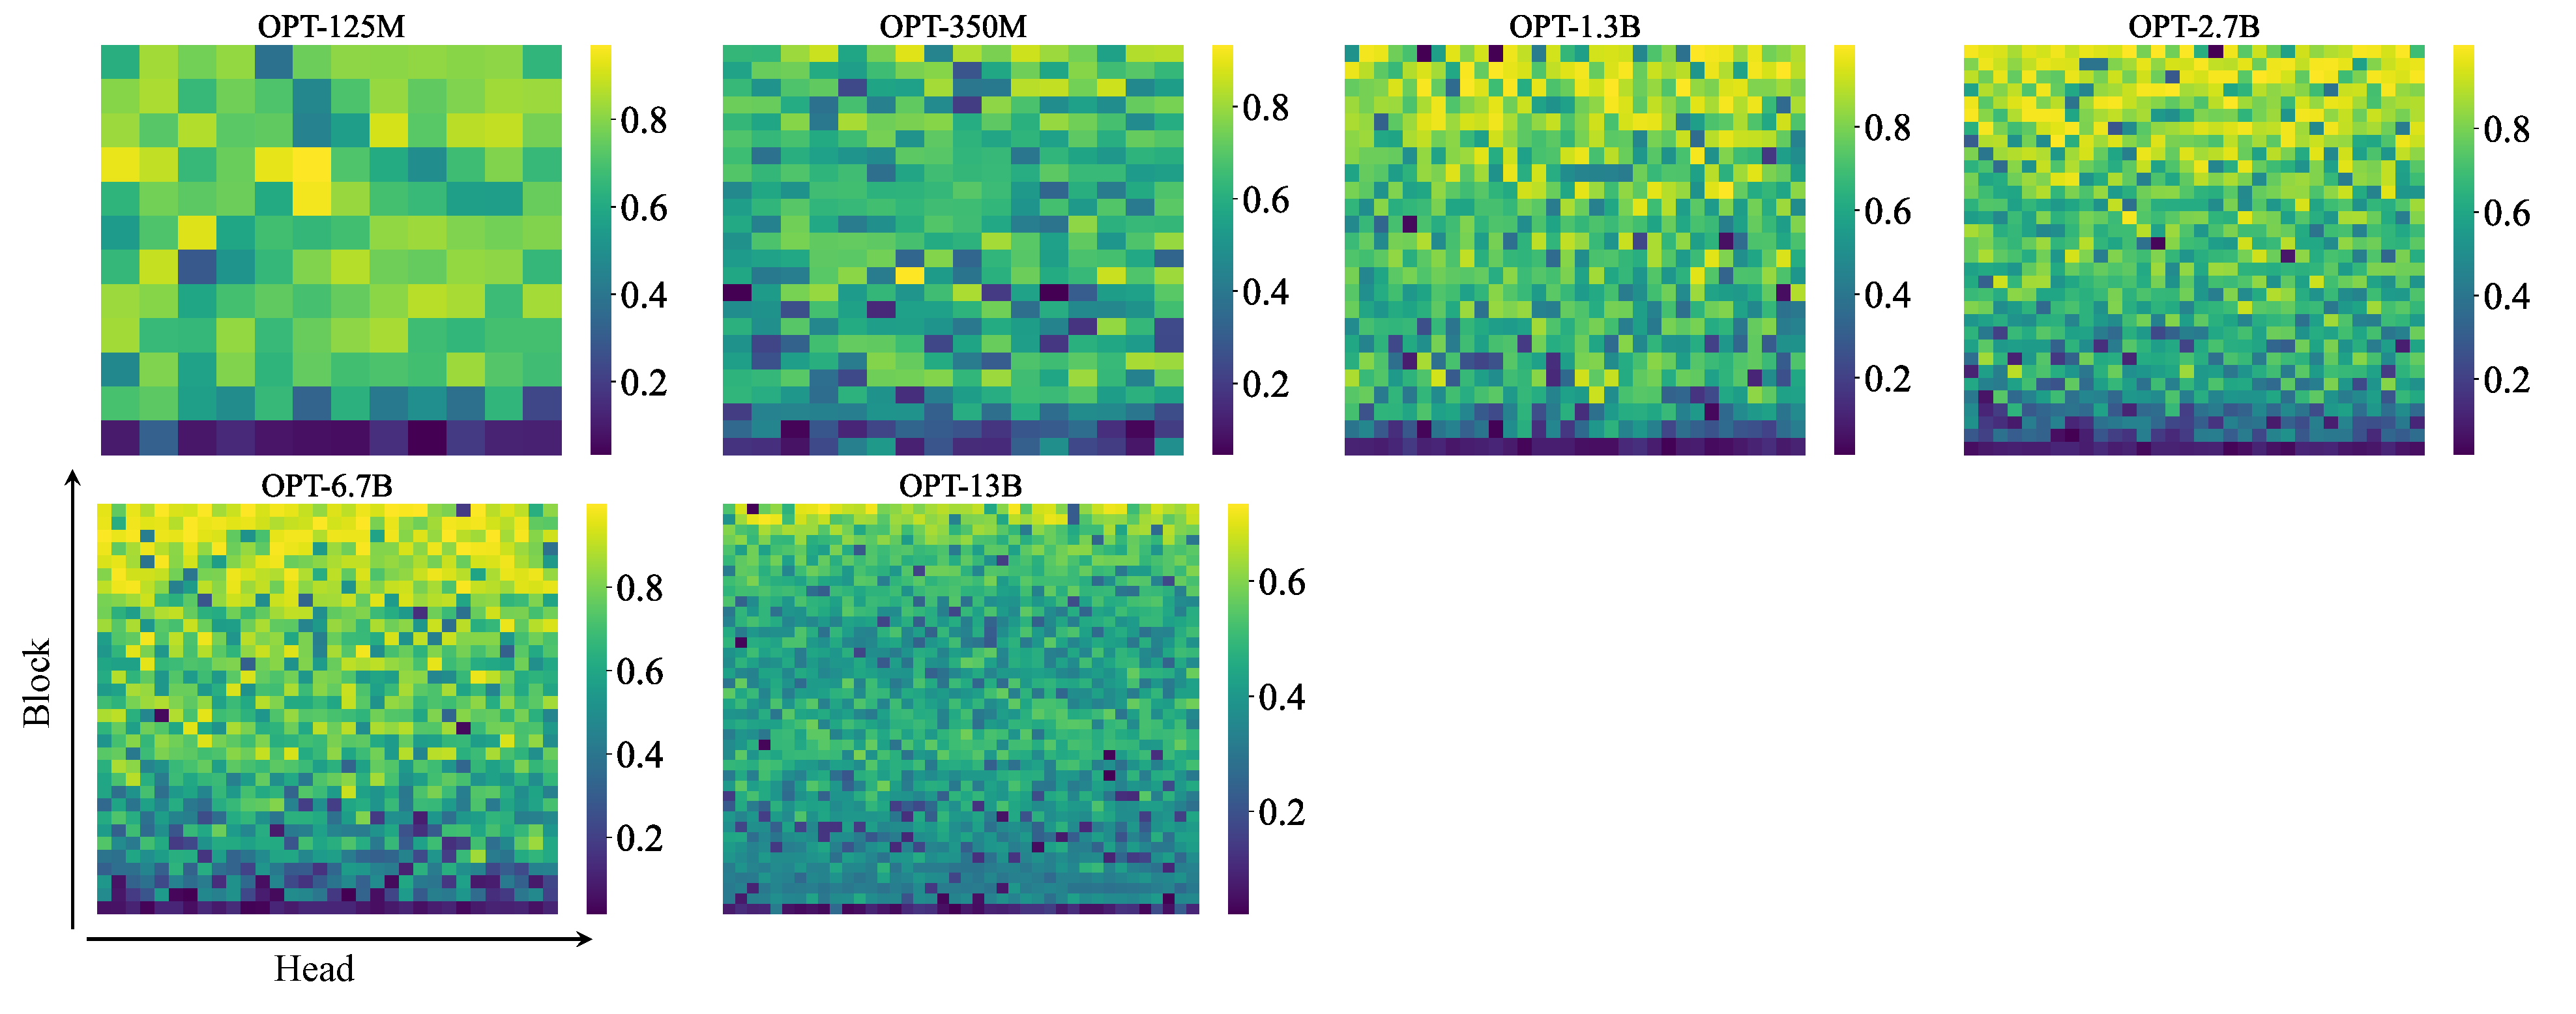
\includegraphics[width=\textwidth]{figures/appendix_layer_head_opt.pdf}
% \vspace{-0.85cm}
% \vspace{-0.2cm}
\caption{Distribution of importance scores for the first token across blocks and heads in the OPT family.\looseness=-1}
% \vspace{-.4cm}
\label{appendix_layer_head_opt}
\end{figure}

\begin{figure}[htbp]
\centering
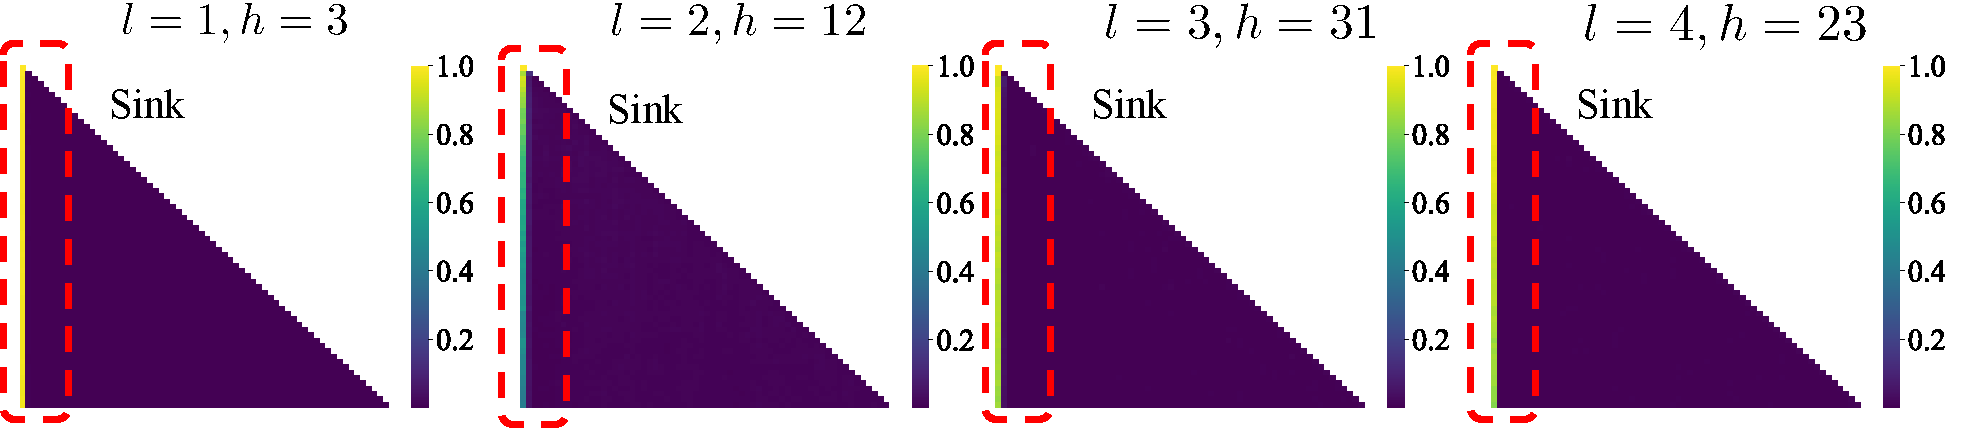
\includegraphics[width=\textwidth]{figures/jamba_v0.1_attention.pdf}
% \vspace{-0.85cm}
% \vspace{-0.2cm}
\caption{Attention sink in Jamba-v0.1.\looseness=-1}
% \vspace{-.4cm}
\label{appendix_sink_jamba_v0.1}
\end{figure}

\begin{figure}[htbp]
\centering
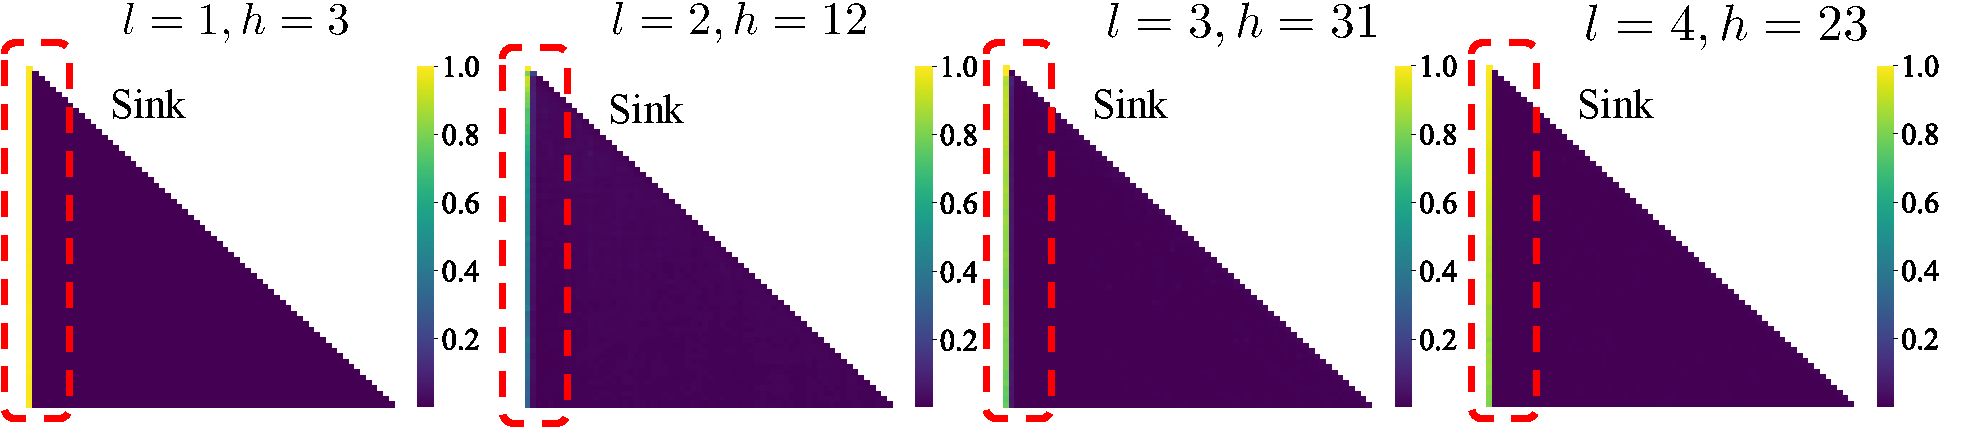
\includegraphics[width=\textwidth]{figures/jamba_1.5_mini_attention.pdf}
% \vspace{-0.85cm}
% \vspace{-0.2cm}
\caption{Attention sink in Jamba-1.5 Mini.\looseness=-1}
% \vspace{-.4cm}
\label{appendix_sink_jamba_1.5_mini}
\end{figure}

\clearpage

\begin{figure}[htbp]
\centering
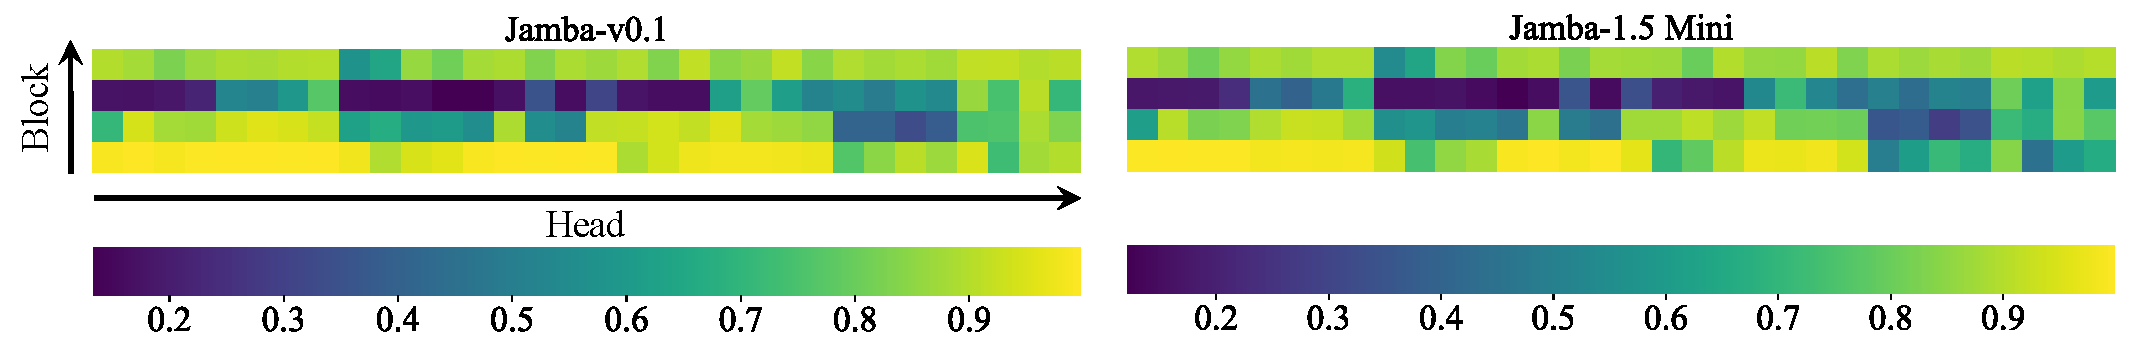
\includegraphics[width=\textwidth]{figures/jamba_layer_head.pdf}
% \vspace{-0.85cm}
% \vspace{-0.2cm}
\caption{Distribution of importance scores for the first token across blocks and heads in the Jamba models.\looseness=-1}
% \vspace{-.4cm}
\label{appendix_layer_head_jamba}
\end{figure}


\subsection{Huggingface links for open-sourced LMs}

% In this section, we provide all huggingface links to the open-sourced LMs we used in this paper.


\begin{table}[htbp]
\vspace{-.2cm}
\caption{Huggingface links for open-sourced LMs we used in this paper.\looseness=-1}
\vspace{-.3cm}
\begin{center}
\begin{tabular}{l|l}
\toprule
Model & Huggingface link \\
\midrule
LLaMA2-7B Base & \href{https://huggingface.co/meta-llama/Llama-2-7b-hf}{meta-llama/Llama-2-7b-hf} \\
LLaMA2-7B Chat & \href{https://huggingface.co/meta-llama/Llama-2-7b-chat-hf}{{meta-llama/Llama-2-7b-chat-hf}} \\
LLaMA2-13B Base & \href{https://huggingface.co/meta-llama/Llama-2-13b-hf}{meta-llama/Llama-2-13b-hf} \\
LLaMA2-13B Chat & \href{https://huggingface.co/meta-llama/Llama-2-13b-chat-hf}{meta-llama/Llama-2-13b-chat-hf} \\
LLaMA3-8B Base & \href{https://huggingface.co/meta-llama/Meta-Llama-3-8B}{meta-llama/Meta-Llama-3-8B} \\
LLaMA3-8B Instruct & \href{https://huggingface.co/meta-llama/Meta-Llama-3-8B-Instruct}{meta-llama/Meta-Llama-3-8B-Instruct} \\
LLaMA3.1-8B Base & \href{https://huggingface.co/meta-llama/Meta-Llama-3.1-8B}{meta-llama/Meta-Llama-3.1-8B} \\
LLaMA3.1-8B Instruct & \href{https://huggingface.co/meta-llama/Meta-Llama-3.1-8B-Instruct}{meta-llama/Meta-Llama-3.1-8B-Instruct} \\
\midrule
GPT2 & \href{https://huggingface.co/openai-community/gpt2}{openai-community/gpt2}\\
GPT2-Medium &\href{https://huggingface.co/openai-community/gpt2-medium}{openai-community/gpt2-medium} \\
GPT2-Large & \href{https://huggingface.co/openai-community/gpt2-large}{openai-community/gpt2-large}\\
GPT2-XL & \href{https://huggingface.co/openai-community/gpt2-xl}{openai-community/gpt2-xl}\\
\midrule
Mistral-7B & \href{https://huggingface.co/mistralai/Mistral-7B-v0.1}{mistralai/Mistral-7B-v0.1}\\
Mistral-7B Instruct & \href{https://huggingface.co/mistralai/Mistral-7B-Instruct-v0.1}{mistralai/Mistral-7B-Instruct-v0.1} \\
\midrule
Pythia-14M & \href{https://huggingface.co/EleutherAI/pythia-14m}{EleutherAI/pythia-14m} \\
Pythia-31M & \href{https://huggingface.co/EleutherAI/pythia-31m}{EleutherAI/pythia-31m} \\
Pythia-70M & \href{https://huggingface.co/EleutherAI/pythia-70m}{EleutherAI/pythia-70m} \\
Pythia-160M & \href{https://huggingface.co/EleutherAI/pythia-160m}{EleutherAI/pythia-160m} \\
Pythia-410M & \href{https://huggingface.co/EleutherAI/pythia-410m}{EleutherAI/pythia-410m} \\
Pythia-1B & \href{https://huggingface.co/EleutherAI/pythia-1b}{EleutherAI/pythia-1b} \\
Pythia-1.4B & \href{https://huggingface.co/EleutherAI/pythia-1.4b}{EleutherAI/pythia-1.4b} \\
Pythia-2.8B & \href{https://huggingface.co/EleutherAI/pythia-2.8b}{EleutherAI/pythia-2.8b} \\
Pythia-6.9B & \href{https://huggingface.co/EleutherAI/pythia-6.9b}{EleutherAI/pythia-6.9b} \\
Pythia-12B & \href{https://huggingface.co/EleutherAI/pythia-12b}{EleutherAI/pythia-12b} \\
\midrule
OPT-125M & \href{https://huggingface.co/facebook/opt-125m}{facebook/opt-125m} \\
OPT-350M & \href{https://huggingface.co/facebook/opt-350m}{facebook/opt-350m} \\
OPT-1.3B & \href{https://huggingface.co/facebook/opt-1.3b}{facebook/opt-1.3b} \\
OPT-2.7B & \href{https://huggingface.co/facebook/opt-2.7b}{facebook/opt-2.7b} \\
OPT-6.7B & \href{https://huggingface.co/facebook/opt-6.7b}{facebook/opt-6.7b} \\
OPT-13B & \href{https://huggingface.co/facebook/opt-13b}{facebook/opt-13b} \\
\midrule
Jamba-v0.1 &  \href{https://huggingface.co/ai21labs/Jamba-v0.1}{ai21labs/Jamba-v0.1} \\
Jamba-1.5 Mini & \href{https://huggingface.co/ai21labs/AI21-Jamba-1.5-Mini}{ai21labs/AI21-Jamba-1.5-Mini} \\
\bottomrule
\end{tabular}
\end{center}
% \vspace{-.2cm}
\label{model_link}
\end{table}


% \subsection{Attention sink metrics for different LLMs}

